% =============================================================================
% Do We Still Need Fine-Tuning for Clinical Text Classification?
% Training-free semantic search vs. fine-tuned transformers (BPD screening)
% =============================================================================
\documentclass[11pt]{article}

\usepackage{graphicx}
\usepackage{authblk}
\usepackage[margin=1in]{geometry}
\usepackage[font=small,skip=4pt]{caption}
\usepackage{float}
\usepackage{microtype}
\usepackage[hyphens]{url}
\usepackage{booktabs}
\usepackage{multirow}
\usepackage{array}
\usepackage{makecell}
\usepackage{xcolor}
\usepackage{amsmath}
\usepackage{amssymb}
\usepackage{enumitem}
\usepackage{tikz}
\usetikzlibrary{shapes.geometric,arrows.meta,positioning,calc,fit,backgrounds}

\usepackage[backend=biber,style=numeric,sorting=none]{biblatex}
\addbibresource{references.bib}
\providecommand{\citealp}[1]{\cite{#1}}

\usepackage{hyperref}
\hypersetup{colorlinks=true,linkcolor=blue!60!black,citecolor=blue!60!black,urlcolor=blue!60!black}

\newcommand{\vbri}{VBRI}
\newcommand{\bpdqac}{BPDQAC}
\newcommand{\dsmv}{DSM-5}
\definecolor{ftblue}{HTML}{2A78D6}
\definecolor{vborange}{HTML}{EB6834}

\title{\textbf{Do We Still Need Fine-Tuning for Clinical Text Classification?
}}

\author[1]{Mehedi Hasan Moon\thanks{mehedi.hasan.moon@ict.mist.ac.bd}}
\author[1]{Md.\ Mahbubur Rahman}
\affil[1]{Department of Computer Science and Engineering, Military Institute of Science and Technology,
Mirpur Cantonment, Dhaka 1216, Bangladesh}
\date{\today}

\begin{document}
\maketitle

% =============================================================================
% ABSTRACT
% =============================================================================
\begin{abstract}
Fine-tuning a pretrained language model is now the usual way to build a text classifier. Large
language models (LLMs) are also used for the same job. Both routes need heavy computing, task-specific
weights and special hardware. This limits their use in low-resource clinical settings. We ask a
simple question: for a classification task, do we really need to fine-tune a model, or can a
frozen embedding model with semantic search do the job? We test this on borderline personality
disorder (BPD) screening. We use \bpdqac{}, a dataset of 3,258 expert-annotated question--answer
pairs from 362 participants. Each participant answered nine open-ended questions based on the
\dsmv{} Criterion A symptoms. We compare eight fine-tuned encoder models (60M to 184M parameters)
with a training-free method that we call Vector-Based Retrieval Inference (\vbri{}). \vbri{}
encodes labelled answers once with a frozen embedding model (\texttt{bge-base-en-v1.5}). It keeps
them in nine criterion-specific, class-balanced vector databases. A new answer is labelled by
similarity-weighted $k$-nearest-neighbour voting. On the same 333 held-out answers, the best
fine-tuned model (ModernBERT) reaches 85.89\% accuracy and 86.57\% BPD sensitivity. \vbri{} needs
no training. It reaches 72.67\% accuracy and 85.07\% BPD sensitivity (57 of 67 BPD answers, against
58 for ModernBERT). With a rule-based suicide-attempt check, it reaches 86.57\%. \vbri{} builds its
index in 12 seconds instead of minutes of GPU training. Its index takes 12.4\,MB, while a fine-tuned
checkpoint takes 264 to 596\,MB. It answers in 2.4\,ms per response and shows the stored answers
behind every decision. Two design choices matter most. Isolating each criterion in its own database
removes the 35.7\% cross-criterion contamination of a single pooled index. Balancing each database
makes the vote fair. Fine-tuning is still better for overall accuracy. But semantic search over an
embedding index is a cheaper and more transparent option when high sensitivity, fast updates and
limited hardware are the main needs.
\end{abstract}

\noindent\textbf{Keywords:} text classification, sentence embeddings, semantic search, vector
database, $k$-nearest neighbours, training-free inference, fine-tuning, large language models,
borderline personality disorder, clinical NLP, resource-constrained deployment.

% =============================================================================
% 1. INTRODUCTION
% =============================================================================
\section{Introduction}\label{sec:intro}

Text classification is a core task in natural language processing (NLP). In health care, it helps
to sort patient messages, flag risk in clinical notes and screen people for mental health problems.
One recipe now dominates. Take a pretrained transformer such as BERT~\cite{devlin2019bert}. Then
fine-tune all of its weights on labelled examples. More recently, large language models (LLMs) have
joined in. They are prompted directly, or fine-tuned, for mental health
prediction~\cite{yang2024mentallama,xu2024mental,guo2024llmreview}. Behind all of this sits one
assumption: a classifier must be \emph{trained} for every new task.

This assumption has a cost. Fine-tuning needs a GPU and many hours of trial and error. Class
imbalance and overfitting must be handled with care. Every task gives a new set of weights. These
must be stored, versioned and retrained when the labels or the data change. The energy and money
cost of training is a known concern in NLP~\cite{strubell2019energy,schwartz2020green}. LLMs make
it worse. They have billions of parameters and often run on remote servers. They also raise privacy
questions when the input is clinical text~\cite{guo2024llmreview}. And they do not clearly win.
Several studies show that small fine-tuned encoders still beat zero-shot and few-shot LLMs on text
classification~\cite{bucher2024finetuned,edwards2024icl}. In mental health, zero-shot ChatGPT did
poorly on suicidality detection~\cite{lamichhane2023chatgpt}.

There is a third option, and it is often missed. Sentence embedding models turn text into dense
vectors. Texts with similar meaning land close together~\cite{reimers2019sbert,xiao2023cpack,muennighoff2023mteb}.
This is the idea behind semantic search and retrieval-augmented generation
(RAG)~\cite{karpukhin2020dpr,lewis2020rag}. Now think of a new patient answer. If it sits close to
many earlier answers that experts marked as BPD-indicative, we can give it the same label. No
gradient update is needed. The ``model'' is a frozen encoder plus a small database of labelled
vectors. We can update it by adding rows. It runs on modest hardware. Each decision can be explained
by showing the stored answers behind it. A recent clinical study found that text embeddings with a
light classifier detected depression in patient narratives better than GPT-4o~\cite{lho2025jama}.

The setting of this study makes these points important. Borderline personality disorder is a severe
condition. It shows as unstable relationships, unstable self-image and unstable emotions, together
with impulsive behaviour~\cite{dsm}. The median prevalence in the general population is about 1.6\%.
It rises to around 10\% in outpatient clinics and 20\% in psychiatric inpatients~\cite{dsm}. Between
40\% and 85\% of people with BPD attempt suicide, and up to 10\% die by
suicide~\cite{paris2001,stone1990,oumaya2008}. Diagnosis usually needs an interview with a licensed
clinician and tools such as the MSI-BPD~\cite{zanarini2003}. Access is a problem. In Bangladesh,
about 90\% of people with a mental health condition do not get treatment~\cite{huque2025}. A
screening tool for this setting must be cheap to build and run. It must be easy to update. It must
be clear to clinicians. And it should run locally, so that sensitive answers never leave the clinic.

So we ask a direct question. \textbf{Do we really need to fine-tune a language model to classify
clinical text, or can semantic search over a frozen embedding model do the job?} We answer it on
\bpdqac{}, a dataset of expert-labelled answers to structured BPD interview questions. We run a
controlled, head-to-head test of two paradigms. Both use the same data and the same test set.
Paradigm A is a set of fine-tuned transformer encoders. Paradigm B is a training-free retrieval
classifier that we call Vector-Based Retrieval Inference (\vbri{}).

The objectives of this work are:
\begin{enumerate}[leftmargin=*,itemsep=2pt]
  \item To compare fine-tuned encoders with retrieval methods on the same held-out clinical answers
        in terms of effectiveness, training time, inference time and storage.
  \item To develop \vbri{}, a training-free classifier that uses a frozen embedding model and nine
        criterion-isolated, class-balanced vector databases.
  \item To analyse why naive semantic search fails and to test, through a $2\times2$ ablation,
        whether criterion isolation and class balancing fix it.
  \item To assess the trade-off between fine-tuning and \vbri{} in accuracy, cost, ease of update
        and explainability.
\end{enumerate}

The paper is organised as follows. Section~\ref{sec:lit} reviews related work and states the
research gap. Section~\ref{sec:dataset} describes the dataset. Section~\ref{sec:method} explains
both methods and the reasons behind each decision. Section~\ref{sec:results} gives the results.
Section~\ref{sec:discussion} discusses what they mean and where they stop. Section~\ref{sec:conclusion}
concludes.

% =============================================================================
% 2. LITERATURE REVIEW
% =============================================================================
\section{Literature Review}\label{sec:lit}

This section follows the path that leads to our question. First, we show how mental health text
classification came to rely on trained and fine-tuned models. Then we look at what LLMs add, and
what they cost. Last, we review the embedding and retrieval methods that make a training-free
option possible.

\subsection{Mental health text classification: from feature engineering to fine-tuning}

Early work detected psychological states from social media posts with classical classifiers. Singh
et al.~\cite{singh2020framework} used NLP preprocessing with Logistic Regression, Support Vector
Machines, Na\"{i}ve Bayes and Decision Trees to detect antisocial behaviour on Twitter. A review by
Harrigian et al.~\cite{harrigian2021state} listed 102 social media mental health datasets. Most came
from Twitter and Reddit. Most studied depression and suicidal ideation. Most used self-reported
labels. These models relied on hand-made features. They struggled with subtle language.

Transformers changed this. Dinu and Moldovan~\cite{dinu2021automatic} fine-tuned BERT, RoBERTa and
XLNet on general Reddit posts and reached up to 81\% accuracy. Jiang et
al.~\cite{jiang-etal-2020-detection} used contextual BERT representations on 17.5 million posts
from users with eight disorders. Haque et al.~\cite{suicidalideationtransformers2020} reported
95.21\% accuracy with RoBERTa for suicidal ideation. Domain-adapted models followed. PsychBERT was
pretrained on mental health literature and social media~\cite{vajre2021psychbert}. MentalBERT and
MentalRoBERTa were pretrained on mental health subreddits~\cite{ji2022mentalbert}. BERT-based models
were also used for early self-harm detection~\cite{martinez2022early}. Reviews of this period agree
on two points~\cite{zhang2022natural,montejo2024survey,greco2023transformer}. Transformers dominate.
And most are trained on social media data with weak labels and little clinical validation. In every
case, a new task meant a new round of training.

\subsection{Personality disorder and BPD detection}

Work on personality disorders follows the same pattern. Jain et al.~\cite{jain2024} fine-tuned BERT
to classify four personality disorders and reached 74.7\% accuracy. Ellouze and
Belguith~\cite{ellouze2022hybrid,ellouze2022deep} combined CNN, BiLSTM and SVM layers to detect
personality disorders from tweets (F1 of 84\%). They later reviewed the move from classical to deep
models~\cite{ellouze2024artificial}. Baqasah et al.~\cite{baqasah2024personality} trained LSTMs on
social media text and reached 89\% accuracy.

Studies on BPD itself are rare. MindTime analysed diary entries with SVM and LSTM classifiers and
reached about 90\% accuracy~\cite{khazbak2021mindtime}. Wang et al.~\cite{wang2020learning} used
language and speech features from 50 non-clinical interviews to separate BPD, bipolar disorder and
healthy controls (AUROC 0.733). None of these studies used answers to structured diagnostic
questions. All of them trained a model for the task.

\subsection{Large language models for mental health: power and price}

LLMs promised to remove task-specific training. MentaLLaMA~\cite{yang2024mentallama} was
instruction-tuned on 105,000 samples. It gives predictions with explanations. Mental-LLM~\cite{xu2024mental}
showed that instruction fine-tuning improves LLMs a lot on mental health prediction. A systematic
review~\cite{guo2024llmreview} found promising results. It also found unstable outputs,
hallucinations, weak privacy control and ethical risks.

On classification itself, the evidence is mixed. Zero-shot ChatGPT reached an F1 of only 0.37 on
suicidality detection~\cite{lamichhane2023chatgpt}. Across many general benchmarks, fine-tuned
``small'' models such as RoBERTa still beat zero-shot GPT-3.5, GPT-4 and Claude
Opus~\cite{bucher2024finetuned}. Fine-tuning a smaller model also beats few-shot prompting of a
larger one~\cite{edwards2024icl}. So LLMs have not removed the need for training. They usually
add the fine-tuning of an even bigger model. Parameter-efficient methods such as
LoRA~\cite{hu2022lora} make this cheaper, but they do not make it go away.

\subsection{Embedding models, semantic search and training-free classification}

A separate line of work produced embedding models that are useful without task-specific training.
Sentence-BERT~\cite{reimers2019sbert} made it practical to compare sentences with cosine similarity.
Later models such as BGE~\cite{xiao2023cpack} learned from large and varied sets of text pairs.
The Massive Text Embedding Benchmark (MTEB)~\cite{muennighoff2023mteb} tests such models on
retrieval, clustering and classification. For classification, it trains a simple classifier on top
of frozen embeddings. Dense retrieval~\cite{karpukhin2020dpr}, fast similarity search with
FAISS~\cite{johnson2019faiss} and retrieval-augmented generation~\cite{lewis2020rag} made vector
databases a standard part of NLP systems.

Nearest-neighbour ideas also have a long history. $k$NN-LM showed that stored neighbours improve
language modelling~\cite{khandelwal2020knnlm}. Deep $k$-Nearest Neighbours used neighbours to make
predictions easier to interpret~\cite{papernot2018dknn}. Li et al.~\cite{li2023revisitknn} showed
that $k$NN improves and calibrates fine-tuned language models. SetFit~\cite{tunstall2022setfit}
reaches strong few-shot results by adapting a sentence encoder with contrastive learning. But it
still trains the encoder and a classification head.

In mental health, nearest-neighbour retrieval over message embeddings has been used for suicide
risk prediction on social media~\cite{fabregat2022clpsych}. Text embeddings with a light classifier
beat GPT-4o for depression detection from patient narratives~\cite{lho2025jama}.

Embeddings also have a known weakness. Sentence encoders often give a sentence and its negation a
very high similarity~\cite{chiang2023heros,cao2025negation}. This matters in clinical screening.
``I have never tried to hurt myself'' and ``I tried to hurt myself'' must not be treated as the same.
Any embedding-based screening tool must be built and checked with this in mind.

\subsection{Research gap and research questions}

Table~\ref{tab:gap} sums up the most relevant work. Three gaps stand out. First, almost all mental
health and BPD classifiers are trained or fine-tuned for their task. The few retrieval-based
systems use social media posts, not structured clinical answers. Second, studies rarely report
effectiveness and computing cost side by side on the same data. So the price of fine-tuning stays
hidden. Third, nobody has looked at why semantic search works or fails on structured interview data,
where several questions share the same emotional words. These gaps leave one basic question open:
\emph{do we really need to fine-tune a language model for a clinical classification task?}

\begin{table}[H]
\centering
\caption{Positioning of this work against representative prior studies.}
\label{tab:gap}
\small
\setlength{\tabcolsep}{4pt}
\resizebox{\textwidth}{!}{%
\begin{tabular}{@{}lllccc@{}}
\toprule
\textbf{Study} & \textbf{Data} & \textbf{Approach} & \makecell{\textbf{Task-specific}\\\textbf{training}} &
\makecell{\textbf{Cost}\\\textbf{reported}} & \makecell{\textbf{Built-in}\\\textbf{evidence}} \\
\midrule
Dinu \& Moldovan~\cite{dinu2021automatic} & Reddit & Fine-tuned BERT/RoBERTa/XLNet & Yes & No & No \\
Ji et al.~\cite{ji2022mentalbert} & Reddit & Domain-pretrained BERT & Yes & No & No \\
Jain et al.~\cite{jain2024} & PD-TXT & Fine-tuned BERT & Yes & No & No \\
Khazbak et al.~\cite{khazbak2021mindtime} & Diaries & SVM / LSTM & Yes & No & No \\
Wang et al.~\cite{wang2020learning} & 50 interviews & Speech + language features & Yes & No & No \\
Yang et al.~\cite{yang2024mentallama} & Social media & Instruction-tuned LLM & Yes & No & Text rationale \\
Lamichhane~\cite{lamichhane2023chatgpt} & Social media & Zero-shot ChatGPT & No & No & No \\
Fabregat et al.~\cite{fabregat2022clpsych} & Social media & ANN retrieval + RNN & Partly & No & No \\
Lho et al.~\cite{lho2025jama} & Patient narratives & Embeddings + XGBoost vs.\ LLM & Yes (head) & No & No \\
\midrule
\textbf{This work} & \textbf{Structured BPD interviews} & \textbf{Frozen embeddings + $k$NN (\vbri{})}
  & \textbf{No} & \textbf{Yes} & \textbf{Retrieved precedents} \\
\bottomrule
\end{tabular}}
\end{table}

We address the gap with three research questions.
\begin{description}[leftmargin=1.2cm,style=nextline,itemsep=2pt]
  \item[RQ1] Can a training-free semantic search classifier reach the BPD sensitivity of fine-tuned
             transformer encoders on structured clinical interview answers?
  \item[RQ2] What does each paradigm cost in training time, inference time and storage? What does
             the training-free approach give up in return?
  \item[RQ3] Which design decisions make semantic search work for criterion-structured clinical
             data?
\end{description}

We use fine-tuned encoders (66M to 184M parameters) as the comparison point. The literature above
shows that they are still the strongest practical classifiers. They usually match or beat prompted
LLMs on classification. If a training-free method can come close to them, it is a fair candidate
to replace the fine-tuning of larger models too.

% =============================================================================
% 3. DATASET
% =============================================================================
\section{The BPDQAC Dataset}\label{sec:dataset}

\bpdqac{} was built for BPD screening from structured interview answers. The interview has 14
questions. We wrote them with guidance from the \dsmv{}~\cite{dsm} and with help from psychologists
and psychiatrists. Nine open-ended questions cover the nine Criterion A symptoms: abandonment
avoidance, unstable relationships, identity disturbance, impulsive behaviour, suicidal and
self-harm behaviour, affective instability, chronic emptiness, inappropriate anger, and paranoid
ideation or dissociation. Five yes/no questions cover the general personality disorder Criteria B
to F. This study uses only the nine open-ended answers.

In total, 362 participants gave consent and completed the interview. This gave 3,258
question--answer pairs. An expert panel assessed each pair. The panel had a licensed psychiatrist, a
clinical psychologist and a trained counsellor. Each pair got one of three labels. \emph{Normal}
means no clinical symptom. \emph{BPD-indicative} means a pathological symptom that fits the \dsmv{}
severity level. \emph{Inconclusive} means mild distress, or too little information to decide.
Semi-supervised label propagation spread the expert labels across the full dataset.

The data are imbalanced (Figure~\ref{fig:data}a). There are 2,195 Normal, 673 BPD and 390
Inconclusive answers. The label mix also changes from question to question
(Figure~\ref{fig:data}b). Abandonment (Q1) and anger (Q8) give the most BPD answers. The suicidal
and self-harm question (Q5) gives the fewest. Later we show that this per-question imbalance is one
of the main reasons why a naive retrieval classifier fails.

\begin{figure}[H]
\centering
\begin{minipage}{0.44\textwidth}\centering
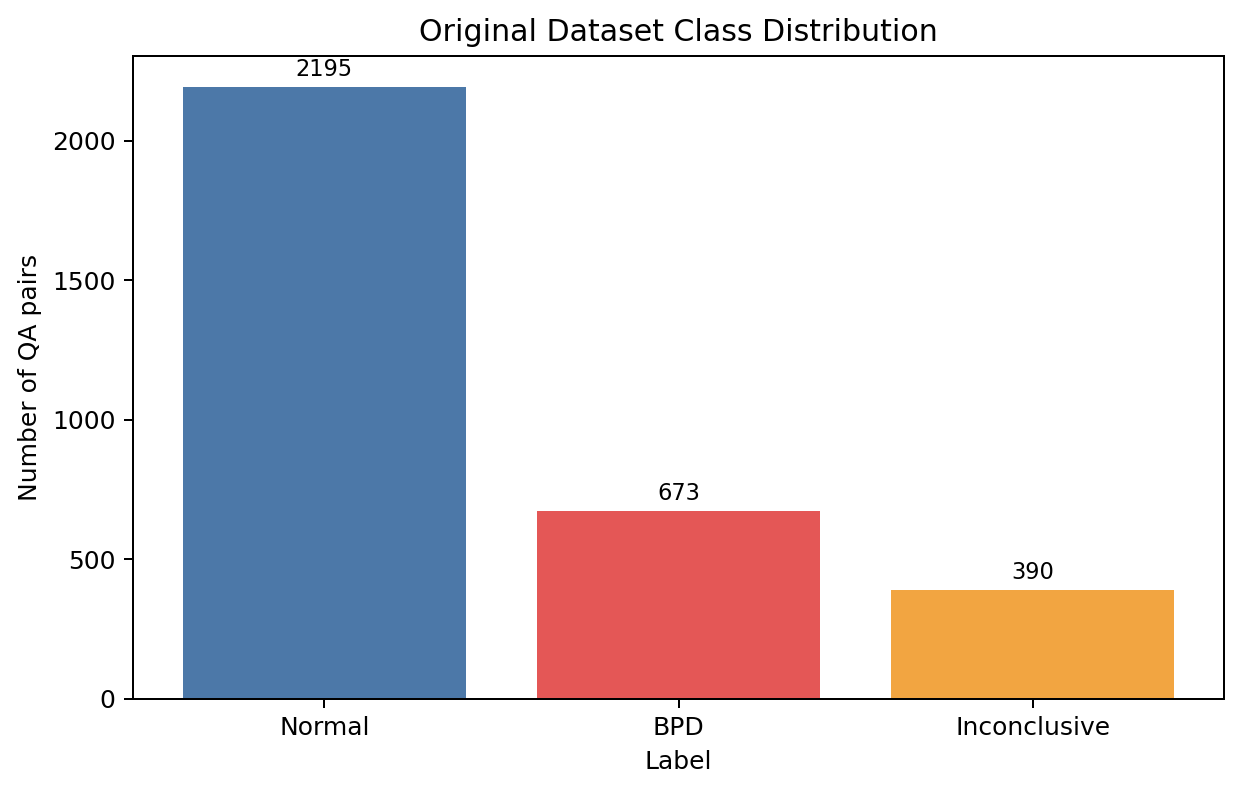
\includegraphics[width=\linewidth]{figures/data_analysis/01_original_class_distribution.png}\\
\small (a) Overall class distribution
\end{minipage}\hfill
\begin{minipage}{0.54\textwidth}\centering
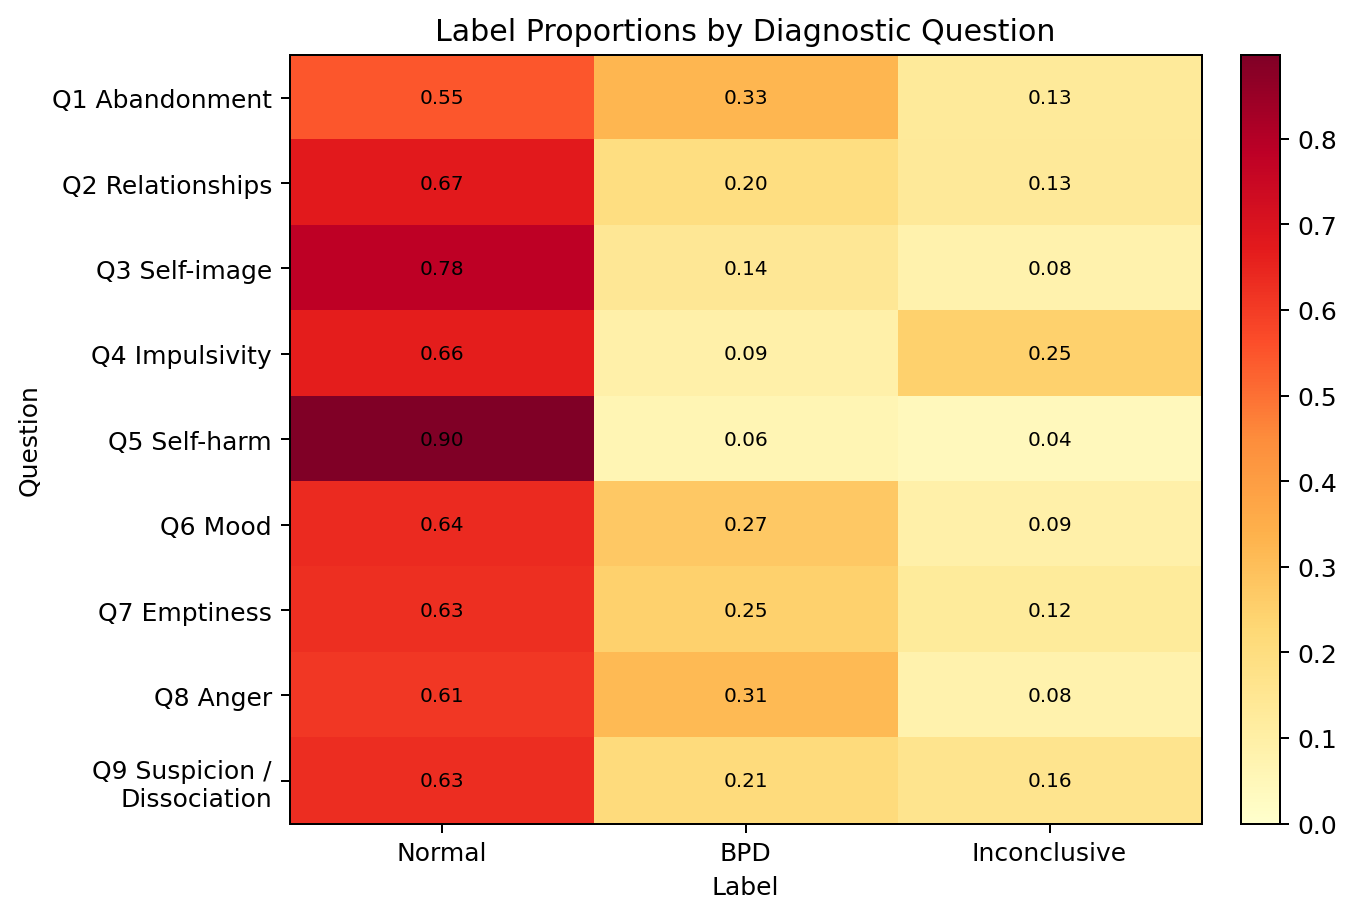
\includegraphics[width=\linewidth]{figures/data_analysis/03_question_label_heatmap_refined.png}\\
\small (b) Label proportions per question
\end{minipage}
\caption{Label structure of \bpdqac{}. The dataset is imbalanced overall. The balance between
Normal, BPD and Inconclusive answers also differs from one diagnostic question to another.}
\label{fig:data}
\end{figure}

\paragraph{Splits and the two training views.}
We split the data into training (2,592 answers), validation (333) and test (333) sets. The
validation and test sets are the same for both paradigms. We never augmented them. The test set has
225 Normal, 67 BPD and 41 Inconclusive answers, 37 per question. Each paradigm then gets a training
view that suits it.
\begin{itemize}[leftmargin=*,itemsep=2pt]
  \item \textbf{Fine-tuning view (5,238 answers).} We augmented the minority classes of the
        training split until each class had 1,746 examples (Figure~\ref{fig:aug}). Balance is set
        over the whole training set. A fine-tuned model learns one decision boundary for all
        questions, so this is the natural choice.
  \item \textbf{Retrieval view (4,050 answers).} \vbri{} votes \emph{inside} one question at a time.
        So balance is set \emph{per question}. Each of the nine databases holds exactly 150 Normal,
        150 BPD and 150 Inconclusive answers. We sub-sampled Normal answers and filled the minority
        classes with augmented answers. Of the 4,050 stored answers, 2,250 are original and 1,800 are
        augmented (651 back-translation, 633 paraphrase, 516 synonym substitution).
\end{itemize}
No augmented text was made from a validation or test answer. A few very short, generic answers
(such as ``nothing significant'') appear in both the training and test sets. There are five such
texts, found in 14 training rows.

\begin{figure}[H]
\centering
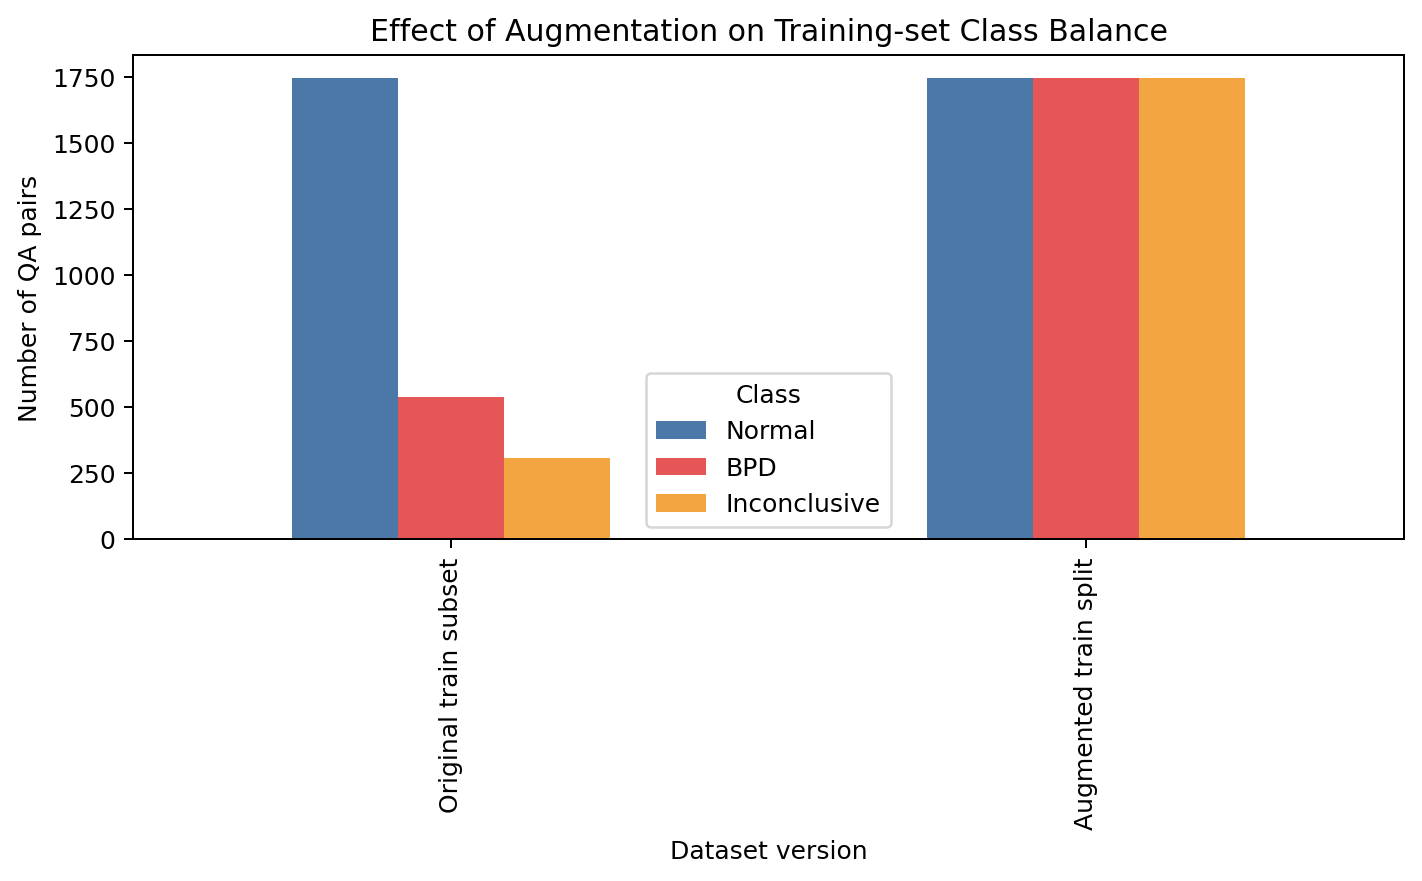
\includegraphics[width=0.7\textwidth]{figures/data_analysis/10_train_augmentation_comparison.png}
\caption{Training-split class balance before and after augmentation (fine-tuning view).}
\label{fig:aug}
\end{figure}

% =============================================================================
% 4. METHODOLOGY
% =============================================================================
\section{Methodology}\label{sec:method}

We compare two ways of building the same three-class classifier (Normal, BPD, Inconclusive). Both
get the same input: a participant's answer to one of the nine questions. Both are scored on the same
333 test answers. Figure~\ref{fig:design} shows the overall study design.

\begin{figure}[H]
\centering
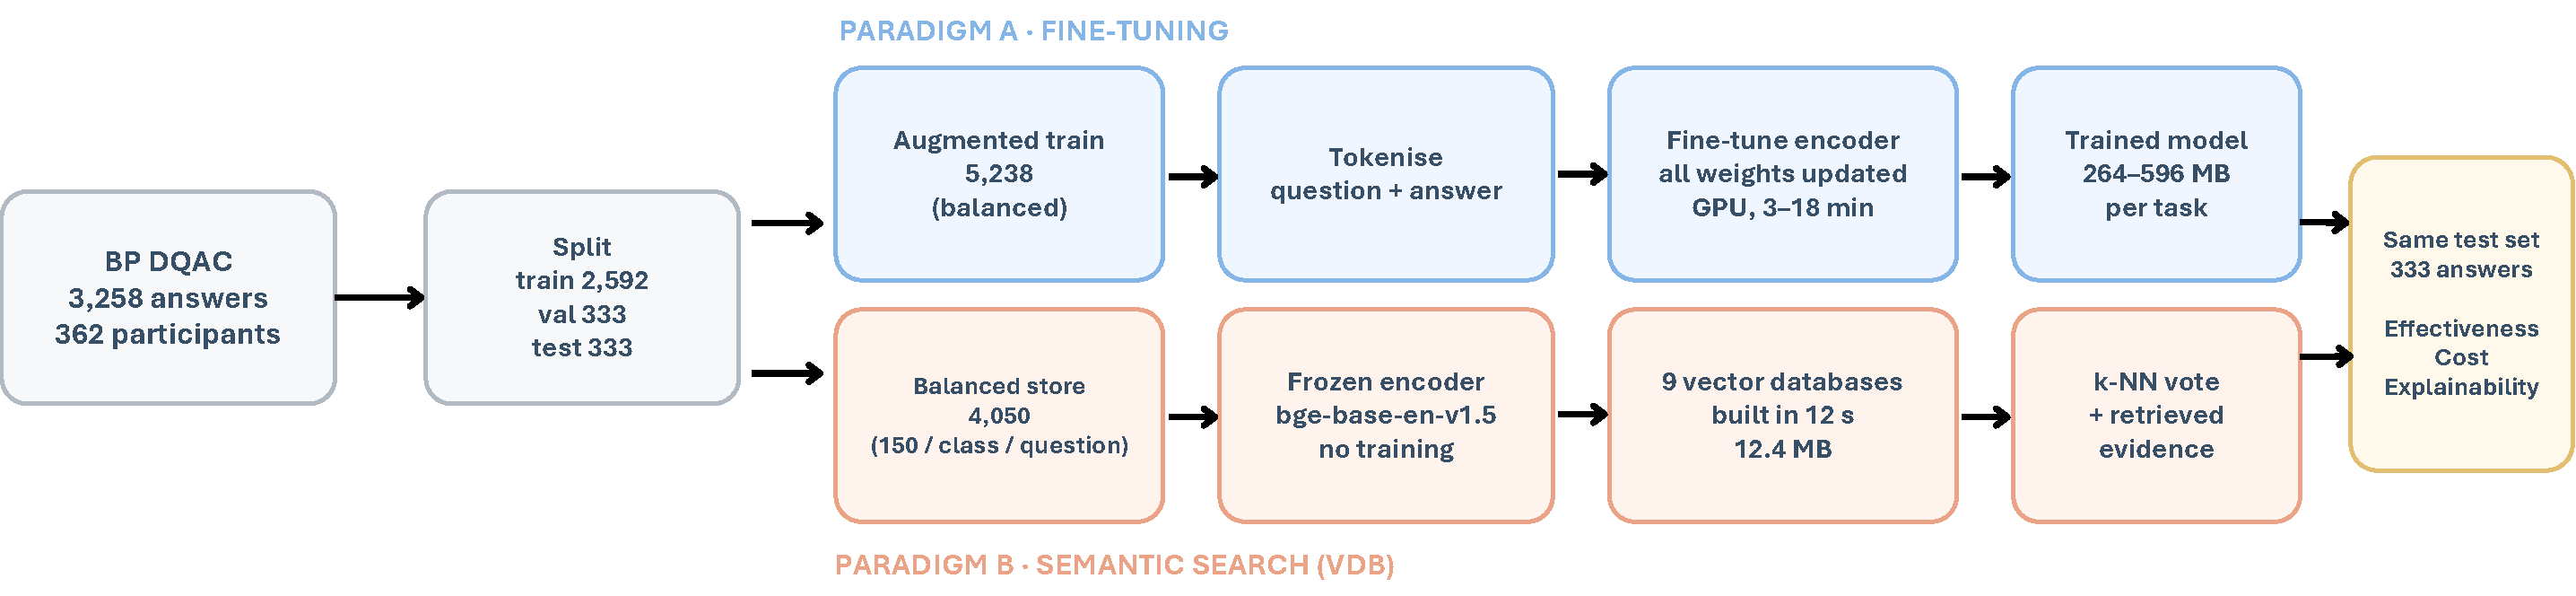
\includegraphics[width=\textwidth]{figures/study_design.pdf}
\caption{Study design. The two paradigms start from the same data and are evaluated on the same
held-out test set. Paradigm A learns new weights for the task. Paradigm B keeps the encoder frozen
and only stores labelled vectors.}
\label{fig:design}
\end{figure}

\subsection{Paradigm A: fine-tuned transformer encoders}

\paragraph{Why this baseline.}
Fine-tuned encoders are the standard way to build a text classifier. As Section~\ref{sec:lit}
shows, they usually match or beat prompted LLMs on classification. So they are the fairest and
strongest comparison for a training-free method.

\paragraph{Workflow.}
Figure~\ref{fig:baseline_workflow} shows the baseline workflow of our project. It has two parts. The
top row covers the data work. The bottom row covers model training and evaluation.

The data work starts with the questionnaire. We prepared it together with psychologists and
psychiatrists. We then collected answers from the participants. Experts checked every label. Then
semi-supervised learning spread these labels to the rest of the data (Section~\ref{sec:dataset}).
Next comes text cleaning. We make the text lower case and remove extra special characters. We expand
contractions. We replace common slang with the help of a hand-made dictionary. NLP preprocessing
then turns the text into model input. The question and the answer go in together as a pair. This
way the model knows which symptom the answer is about. The last step in the top row is class
imbalance. We used oversampling and text augmentation, on the training split only. (We also tried
weighted cross-entropy loss during development. The results here use the augmented training set.)

\begin{figure}[H]
\centering
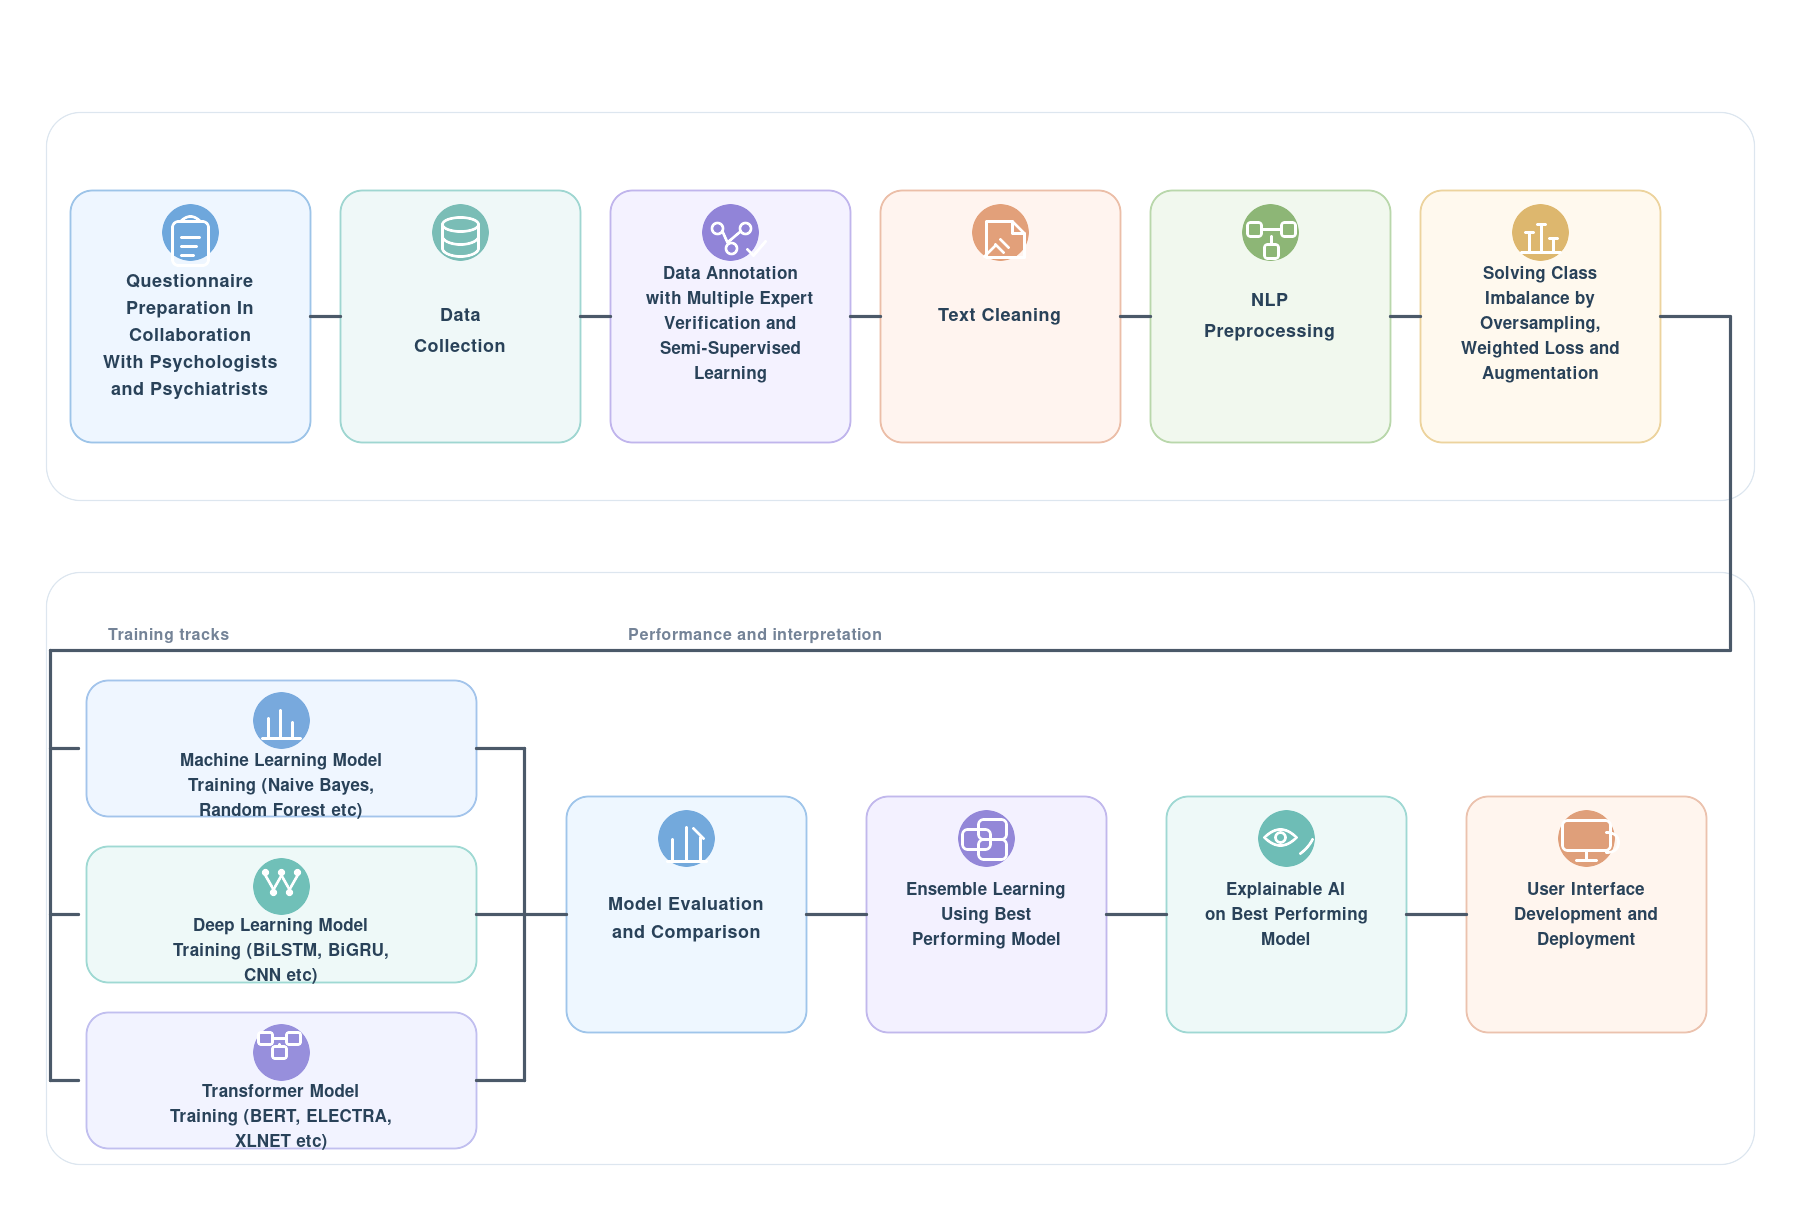
\includegraphics[width=0.98\textwidth]{figures/methodology_workflow_v4.png}
\caption{Baseline methodology workflow of the project. The upper row shows dataset construction and
preparation. The lower row shows model training, evaluation and deployment. This paper uses the
transformer track and the model evaluation step.}
\label{fig:baseline_workflow}
\end{figure}

The bottom row shows three training tracks: classical machine learning, deep learning and
transformers. This paper uses only the transformer track. The model evaluation step then scores all
models on the same test set. Ensemble learning, explainable AI and the user interface are later
stages of the wider project. They are outside the experiments reported here.

\paragraph{Models.}
We fine-tuned eight pretrained models. They cover different design ideas: BERT-base
(110M parameters)~\cite{devlin2019bert}, DistilBERT (66M, a distilled BERT)~\cite{sanh2019distilbert},
RoBERTa-base (125M), ELECTRA-base (110M), XLNet-base (117M), DeBERTa-v3-base (184M),
ModernBERT-base (149M, a recent encoder with longer context and faster
inference)~\cite{warner2024modernbert}, and T5-small (60M, an encoder--decoder). For the encoder
models, a linear layer with three outputs sits on top of the pooled representation. The whole
network is trained with cross-entropy loss. For T5, the input is written as a prompt,
\texttt{trinary classification: <question> </s> <answer>}, and the model generates the label.

\paragraph{Training decisions.}
We trained all models with the Hugging Face \texttt{Trainer} on the 5,238-answer augmented split.
We allowed at most 15 epochs. The effective batch size was 16 (we used gradient accumulation where
memory was short). The learning rate was $5\times10^{-6}$ for BERT, DistilBERT, RoBERTa, ELECTRA
and XLNet. It was $2\times10^{-5}$ for DeBERTa-v3 and ModernBERT, and $5\times10^{-5}$ for T5.
Training stopped early if the validation loss did not improve for two epochs. We kept the checkpoint
with the lowest validation loss. Only the validation set was used to choose models. The test set
was used once, for the final scores. All runs used a single NVIDIA Tesla T4 GPU.

\subsection{Paradigm B: Vector-Based Retrieval Inference (\vbri{})}

\paragraph{Why semantic search.}
The idea behind \vbri{} is simple. An embedding model already puts answers with similar meaning
close together. Experts have already labelled many answers. We store these. To classify a new
answer, we look up its closest stored answers and let them vote. Nothing is trained. The only
``learning'' is writing labelled vectors into a database. This gives four practical benefits for
clinical screening on limited hardware. (1) There is no GPU training. (2) One frozen encoder can
serve any number of tasks. (3) We update the system by adding or removing rows, not by retraining.
(4) Every prediction has a built-in explanation, since the retrieved answers can be shown to the
clinician. Figure~\ref{fig:vbri_arch} shows the full architecture.

\begin{figure}[H]
\centering
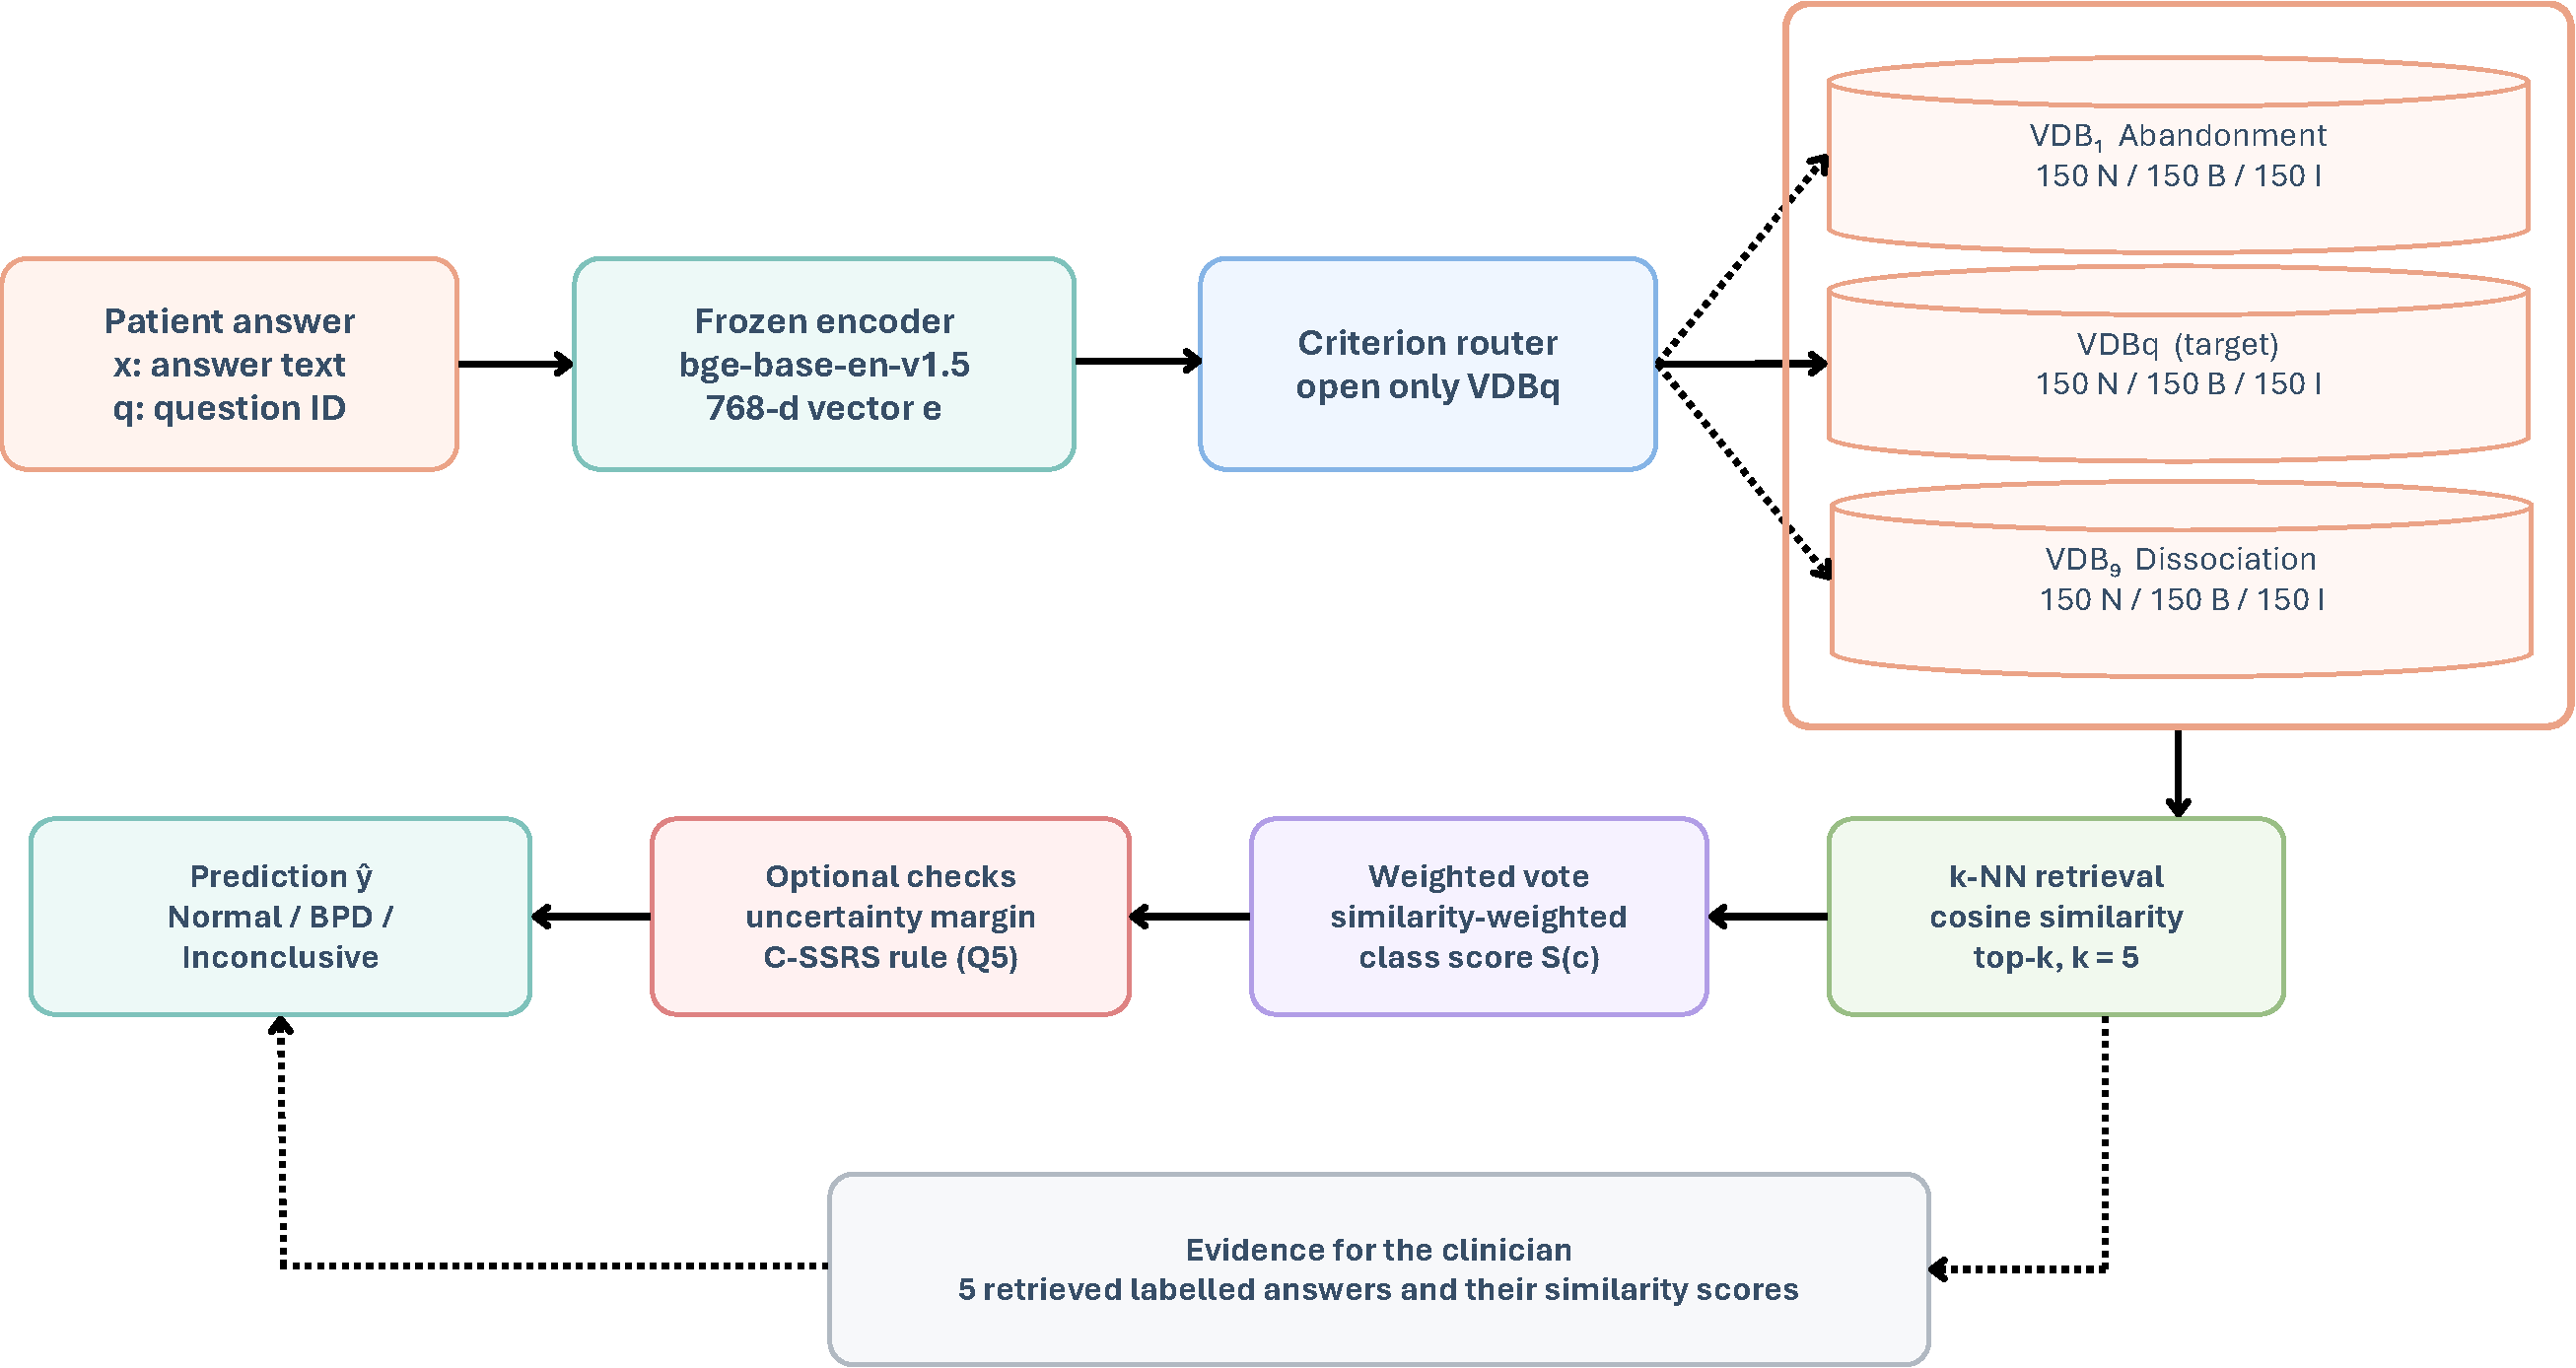
\includegraphics[width=0.92\textwidth]{figures/vbri_architecture.pdf}
\caption{\textbf{\vbri{} architecture.} An answer is encoded by a frozen embedding model and sent
only to the vector database of its own criterion. The top-$k$ most similar stored answers vote,
weighted by similarity. The retrieved answers double as an explanation of the decision.}
\label{fig:vbri_arch}
\end{figure}

\paragraph{Step 1: encoding with a frozen model.}
Every stored answer and every new answer is encoded once with \texttt{BAAI/bge-base-en-v1.5}
(109M parameters)~\cite{xiao2023cpack}. It gives 768-dimensional, unit-length vectors. We tested
four encoders (MiniLM, MPNet, PubMedBERT and BGE). BGE gave the best retrieval results
(Section~\ref{sec:results}), so we chose it. We encode the answer alone. Adding the question text to
every vector made all answers to one question look alike. It lowered accuracy for three of the four
encoders (question+answer vs.\ answer-only accuracy: BGE 45.7\% vs.\ 65.5\%, PubMedBERT 59.5\% vs.\
61.6\%, MiniLM 59.5\% vs.\ 60.7\%). MPNet was the exception (67.6\% vs.\ 64.3\%).

\paragraph{Step 2: one vector database per criterion (decision: isolation).}
Our first version kept all answers in one pooled index. It failed. Answers to different questions
share the same emotional words, such as ``empty'', ``hurt'', ``alone'' and ``angry''. So an answer
about anger often pulled neighbours from the emptiness or mood-instability questions. We now build
nine separate databases, $VDB_1$ to $VDB_9$. Each new answer goes only to the database of its own
question. In a structured interview the question is always known. So this routing is exact and
costs nothing.

\paragraph{Step 3: equal classes in every database (decision: balance).}
A $k$NN vote leans toward whichever class has more stored examples nearby. Inside one criterion, the
natural imbalance can be large. For example, the suicidal behaviour criterion had 259 Normal but
only 54 BPD answers in the augmented training data. So we fill each database with exactly 150
Normal, 150 BPD and 150 Inconclusive answers. This gives 450 per database and 4,050 in total
(Section~\ref{sec:dataset}).

\paragraph{Step 4: similarity-weighted $k$NN vote.}
Take a new answer with embedding $\mathbf{e}$ to question $q$. We compute the cosine similarity
$s_j = \mathbf{e}^\top \mathbf{e}_j$ to every vector in $VDB_q$. We keep the $k$ most similar and
score each class $c$ as
\begin{equation}
S(c) = \sum_{j \in \mathcal{N}_k} \max(s_j, 0)\cdot \mathbb{1}[y_j = c].
\label{eq:voting}
\end{equation}
The class with the highest score is the prediction. Weighting by similarity gives close neighbours
more say than distant ones. We use $k=5$. Results are stable for $k$ between 3 and 7
(Figure~\ref{fig:ksweep}).

\paragraph{Step 5 (optional): uncertainty margin.}
Sometimes the two best classes get almost the same score. Then the evidence is truly mixed. The
calibrated variant turns the scores into class proportions $P(c)=S(c)/\sum_{c'}S(c')$. It returns
Inconclusive when $P_{(1)}-P_{(2)} < \delta$. Otherwise it returns BPD if $P(\text{BPD})\ge\theta$,
and the larger of Normal and Inconclusive if not. We use $\delta=0.05$ and $\theta=0.45$.

\paragraph{Step 6 (optional): suicide-attempt safety rule.}
Embeddings can miss short but critical statements, and negation (Section~\ref{sec:lit}). For the
suicidal and self-harm criterion only, the hybrid variant uses a small set of regular expressions.
They are based on the ``actual attempt'' categories of the Columbia--Suicide Severity Rating Scale
(C-SSRS)~\cite{posner2011cssrs}, for example ``tried to hang myself'' or ``swallowed pills''. If a
pattern matches and the vote says Normal, we change the prediction to BPD. The rule can only move a
prediction toward the safer, positive class.

\paragraph{What is and is not tuned.}
\vbri{} has no trainable parameters. It does have three settings: $k$, $\delta$ and $\theta$. In our
experiments, we chose these by sweeping over the held-out split. We added the C-SSRS rule after we
looked at one missed test case. For a fair comparison, we therefore treat the \emph{raw}
configuration (isolation + balance + $k=5$, no margin, no rule) as the main training-free result.
The calibrated and hybrid variants are exploratory. Their gains should be confirmed on new data.

\subsection{Baselines inside Paradigm B}

To show which parts of \vbri{} matter, we also test simpler retrieval classifiers. They use one
pooled index for all questions. We tried dense retrieval with MiniLM, MPNet, PubMedBERT and BGE
encoders (with answer-only or question+answer text). We also tried two lexical methods, BM25 and
TF-IDF, both with $k=5$. These baselines use the same voting rule as Equation~\eqref{eq:voting}.

\subsection{Evaluation protocol}

\paragraph{Effectiveness.} We report accuracy, macro F1 (which weights the three classes equally),
weighted F1, BPD F1 and BPD sensitivity (the recall of the BPD class). For screening, BPD
sensitivity is the most important number. A missed BPD answer is a person who may not be referred
for assessment. We also report a binary BPD-versus-rest view. It has specificity, positive and
negative predictive values (PPV, NPV) and the diagnostic odds ratio (DOR).

\paragraph{Cost.} We report three things. (i) \emph{Training or index-build time}: the wall-clock
time of the \texttt{Trainer} run, or the time to encode all stored answers. (ii) \emph{Inference
time per answer}: measured on the T4 GPU with batched inputs. For fine-tuned models, this is the
evaluation runtime over 333 answers divided by 333. For \vbri{}, it is the query encoding time plus
the search time. (iii) \emph{Task-specific storage}: what must be kept for each task. This is the
fp32 model weights for fine-tuning and the vector index for \vbri{}. The \vbri{} encoder is shared
and frozen, so we do not count it as task-specific.

\paragraph{Contamination.} For pooled retrieval, we measure the share of the top-$k$ neighbours that
come from a different question than the query. For \vbri{}, this is 0\% by design.

\paragraph{Statistics.} We compare paired predictions with McNemar's test~\cite{mcnemar1947}. We
report both the asymptotic and the exact binomial $p$-values.

% =============================================================================
% 5. RESULTS
% =============================================================================
\section{Results}\label{sec:results}

% TODO(rerun): training times, inference times and the fine-tuned test scores below come from saved
% model artefacts and logs of earlier sessions. Replace them after the clean baseline rerun.

\subsection{How the fine-tuned models learned}

Figure~\ref{fig:loss} shows the training and validation loss of each fine-tuned model. For most
models, the training loss keeps falling. The validation loss stops improving after 2 to 6 epochs.
This is the usual sign of overfitting on a small dataset. Early stopping kept the best checkpoint
(dotted line). ModernBERT reached its best validation loss after only two epochs. DeBERTa-v3 did not
learn. Its training loss stayed almost flat, and it predicted every test answer as Normal. T5 has
a different loss scale because it uses a generative sequence loss.

\begin{figure}[H]
\centering
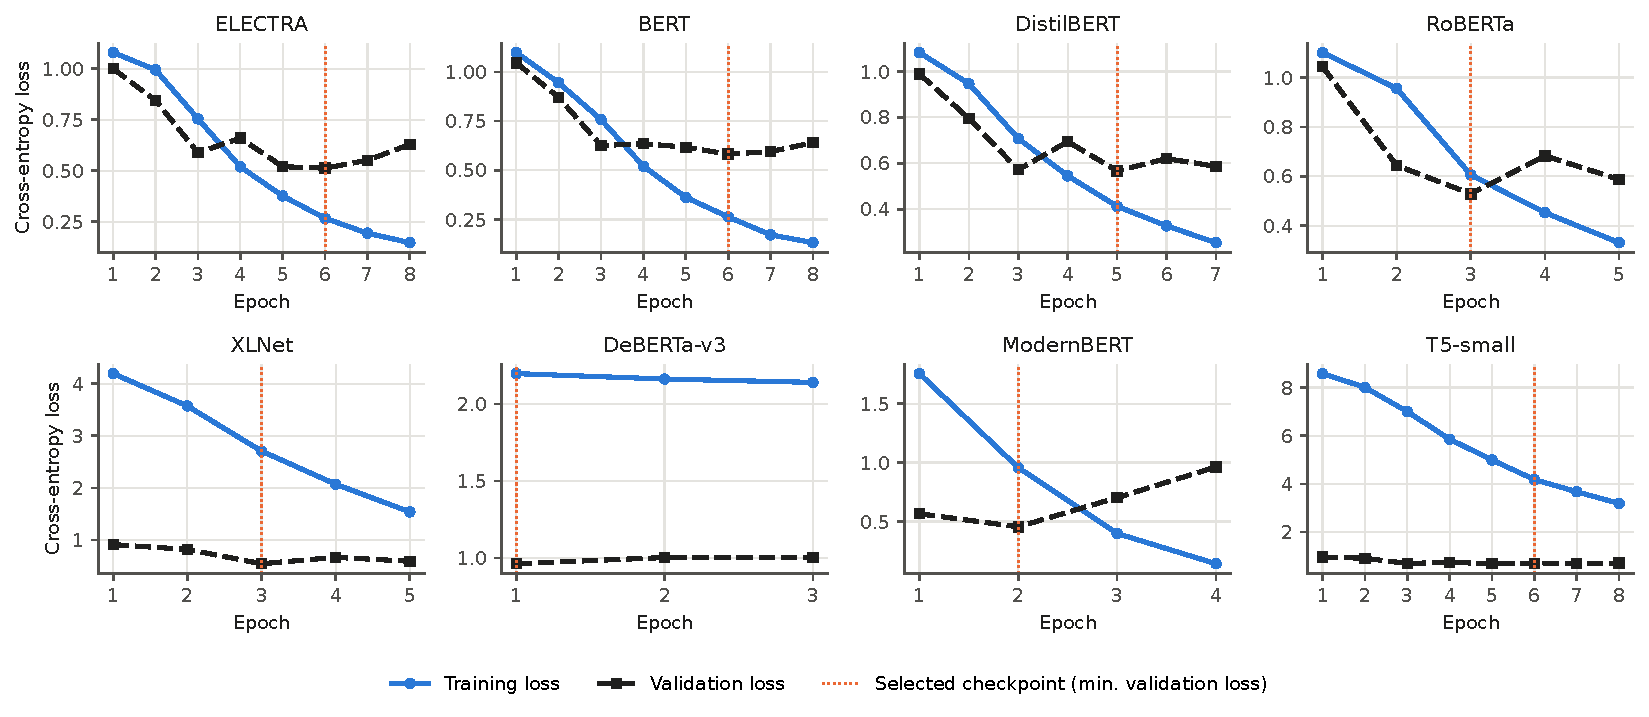
\includegraphics[width=\textwidth]{figures/generated/ft_loss_curves.pdf}
\caption{Training and validation loss per epoch for the eight fine-tuned models (Tesla T4). The
dotted line marks the checkpoint with the lowest validation loss. This checkpoint was kept for
testing.}
\label{fig:loss}
\end{figure}

Table~\ref{tab:encoder_results} and Figure~\ref{fig:ft_cm} give the test results. ModernBERT is the
best model. It has 85.89\% accuracy, 80.25\% macro F1 and 86.57\% BPD sensitivity. It was also the
fastest to train (179\,s). ELECTRA reached the same BPD sensitivity with slightly lower accuracy.
A bigger model is not always better. DeBERTa-v3 is the largest, and it collapsed to the majority
class. T5-small failed to separate the classes.

\begin{table}[H]
\centering
\caption{Fine-tuned encoders on the \bpdqac{} test set ($N=333$). Training time is the
\texttt{Trainer} wall-clock time on one Tesla T4, including all epochs up to early stopping.}
\label{tab:encoder_results}
\small
\setlength{\tabcolsep}{4pt}
\renewcommand{\arraystretch}{1.1}
\resizebox{\textwidth}{!}{%
\begin{tabular}{@{}lccccccc@{}}
\toprule
\textbf{Model} & \textbf{Params} & \textbf{Train time} & \textbf{Accuracy} &
\textbf{Weighted F1} & \textbf{Macro F1} & \textbf{BPD F1} & \textbf{BPD Sens.} \\
\midrule
ModernBERT-base & 149M & 179\,s (3.0 min)  & \textbf{85.89} & \textbf{86.16} & \textbf{80.25} & \textbf{77.85} & \textbf{86.57} \\
ELECTRA-base    & 110M & 1,062\,s (17.7 min) & 83.48 & 83.90 & 77.43 & 76.32 & \textbf{86.57} \\
RoBERTa-base    & 125M & 668\,s (11.1 min)   & 81.08 & 81.96 & 74.65 & 73.55 & 85.07 \\
BERT-base       & 110M & 1,066\,s (17.8 min) & 79.58 & 80.28 & 74.80 & 69.23 & 80.60 \\
XLNet-base      & 117M & 666\,s (11.1 min)   & 77.48 & 78.32 & 71.01 & 65.90 & 85.07 \\
DistilBERT      & 66M  & 475\,s (7.9 min)    & 74.77 & 76.14 & 69.67 & 65.88 & 83.58 \\
DeBERTa-v3-base & 184M & 431\,s (7.2 min)    & 67.57 & 54.49 & 26.88 & 0.00  & 0.00  \\
T5-small        & 60M  & 1,227\,s (20.5 min) & 41.44 & 42.80 & 28.28 & 25.44 & 43.28 \\
\bottomrule
\end{tabular}}
\end{table}

\begin{figure}[H]
\centering
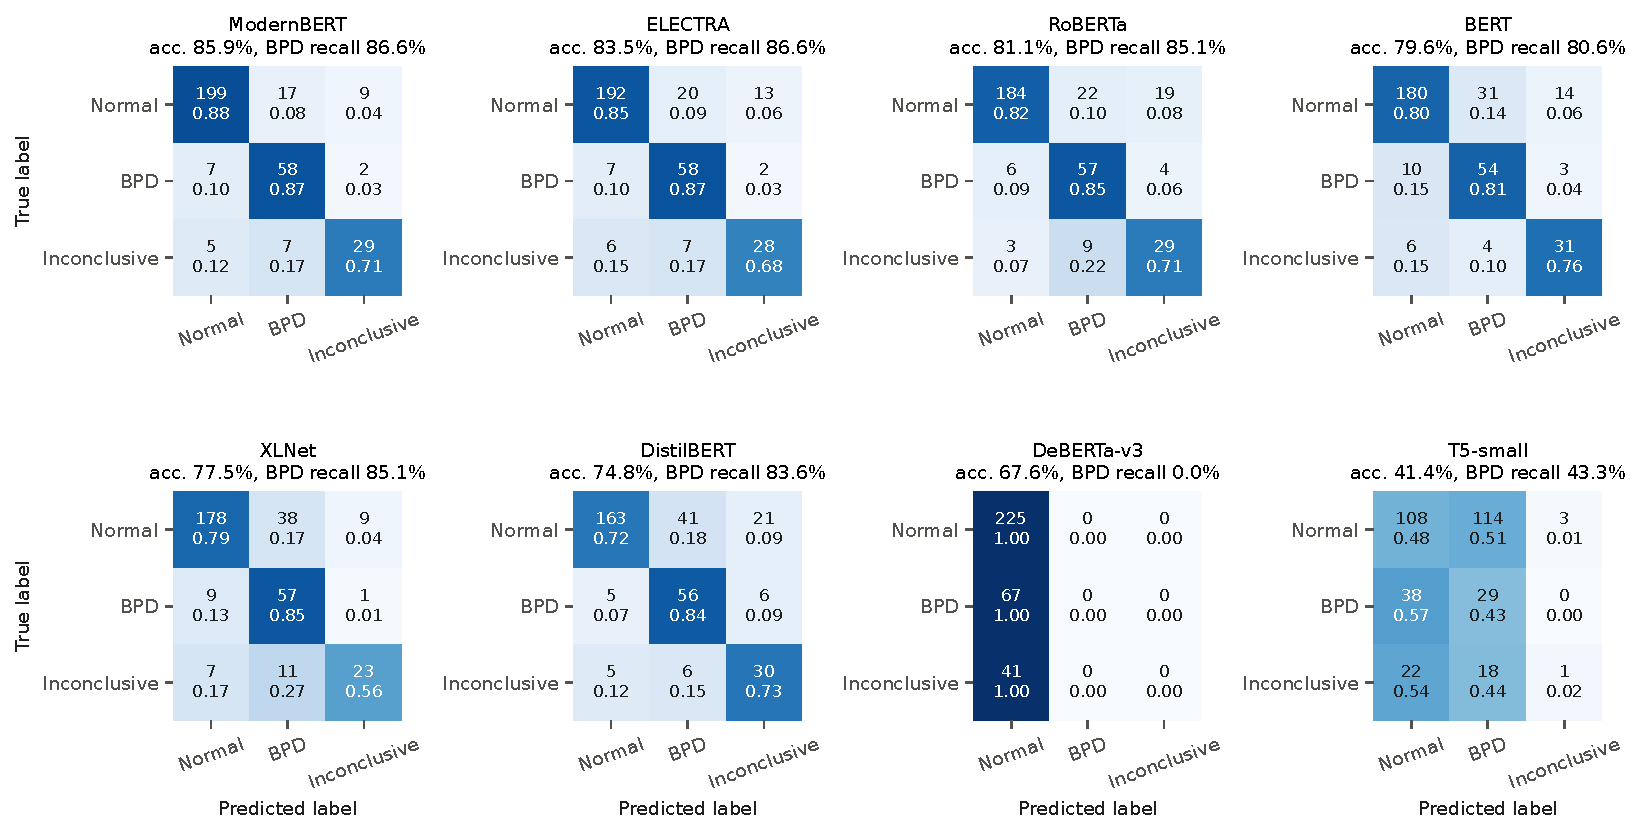
\includegraphics[width=\textwidth]{figures/generated/ft_confusion_matrices.pdf}
\caption{Test confusion matrices of the fine-tuned models (counts and row-normalised
proportions). The best models find most BPD answers. They confuse some Inconclusive answers with
the other two classes.}
\label{fig:ft_cm}
\end{figure}

\subsection{Choosing the encoder and the input text}\label{sec:encoder_text}

We first compared four frozen encoders, each with two input texts: question plus answer, and the
answer alone. All eight runs used one pooled index of the 4,279 augmented training answers and the
same 333 test answers. The $k=3$ nearest neighbours voted, with inverse-frequency class weights.
For BGE, each query also carried a short instruction prefix. Figure~\ref{fig:encoder_text} shows
the results. With the answer alone, BGE was the best encoder (65.47\% accuracy, 57.07\% macro F1).
MPNet followed in accuracy (64.26\%), then PubMedBERT (61.56\%) and MiniLM (60.66\%). The highest
score of all eight runs came from MPNet with question plus answer (67.57\% accuracy, 57.28\% macro
F1), slightly above BGE with the answer alone.

\begin{figure}[H]
\centering
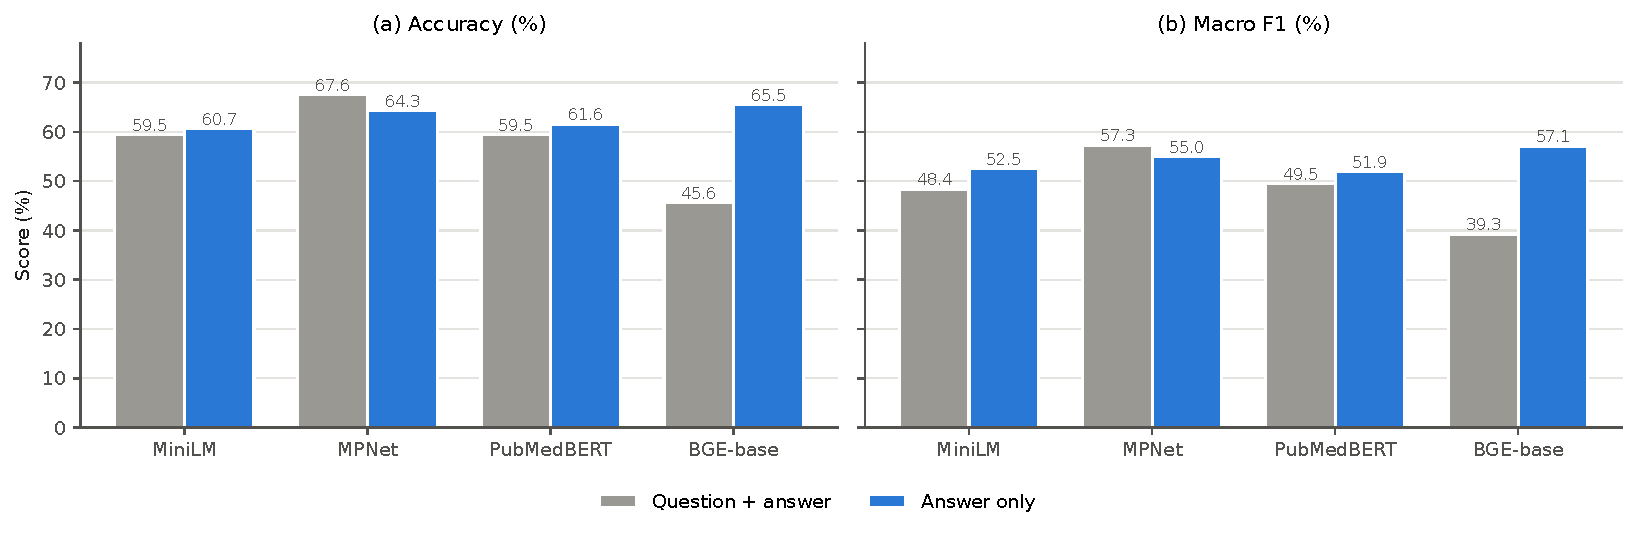
\includegraphics[width=\textwidth]{figures/generated/encoder_input_text.pdf}
\caption{Effect of the input text on four frozen encoders (pooled index, $k=3$, class-weighted
vote, $N=333$). (a) Accuracy. (b) Macro F1.}
\label{fig:encoder_text}
\end{figure}

Adding the question text lowered both accuracy and macro F1 for three of the four encoders. The
drop was large for BGE, from 65.47\% to 45.65\% accuracy. It was small for PubMedBERT (61.56\% to
59.46\%) and MiniLM (60.66\% to 59.46\%), where it amounts to only a few test answers. MPNet moved
the other way, from 64.26\% to 67.57\%. So the effect depends on the encoder. A likely reason for
the drop is that all answers to one question share the same question text, which pulls their
vectors together and hides the differences between the answers. We did not test this explanation
directly. Since \vbri{} uses BGE, it encodes the answer alone.

\subsection{Why naive semantic search fails: cross-criterion contamination}

The simplest semantic search classifier uses one pooled BGE index over all questions. It reaches
only 67.87\% accuracy and 59.52\% macro F1 (Table~\ref{tab:master}). Figure~\ref{fig:contam}b shows
why. On average, 35.7\% of the five retrieved neighbours come from a \emph{different} question than
the query. For abandonment (Q1) it is 44.3\%. These neighbours carry labels that were given for a
different symptom. So part of the vote is based on the wrong evidence. A different encoder does
not fix this. All pooled dense and lexical baselines show 34.8\% to 38.2\% contamination. Their
accuracy stays between 59.8\% and 67.9\%. The problem is the structure of the index, not the encoder.

\begin{figure}[H]
\centering
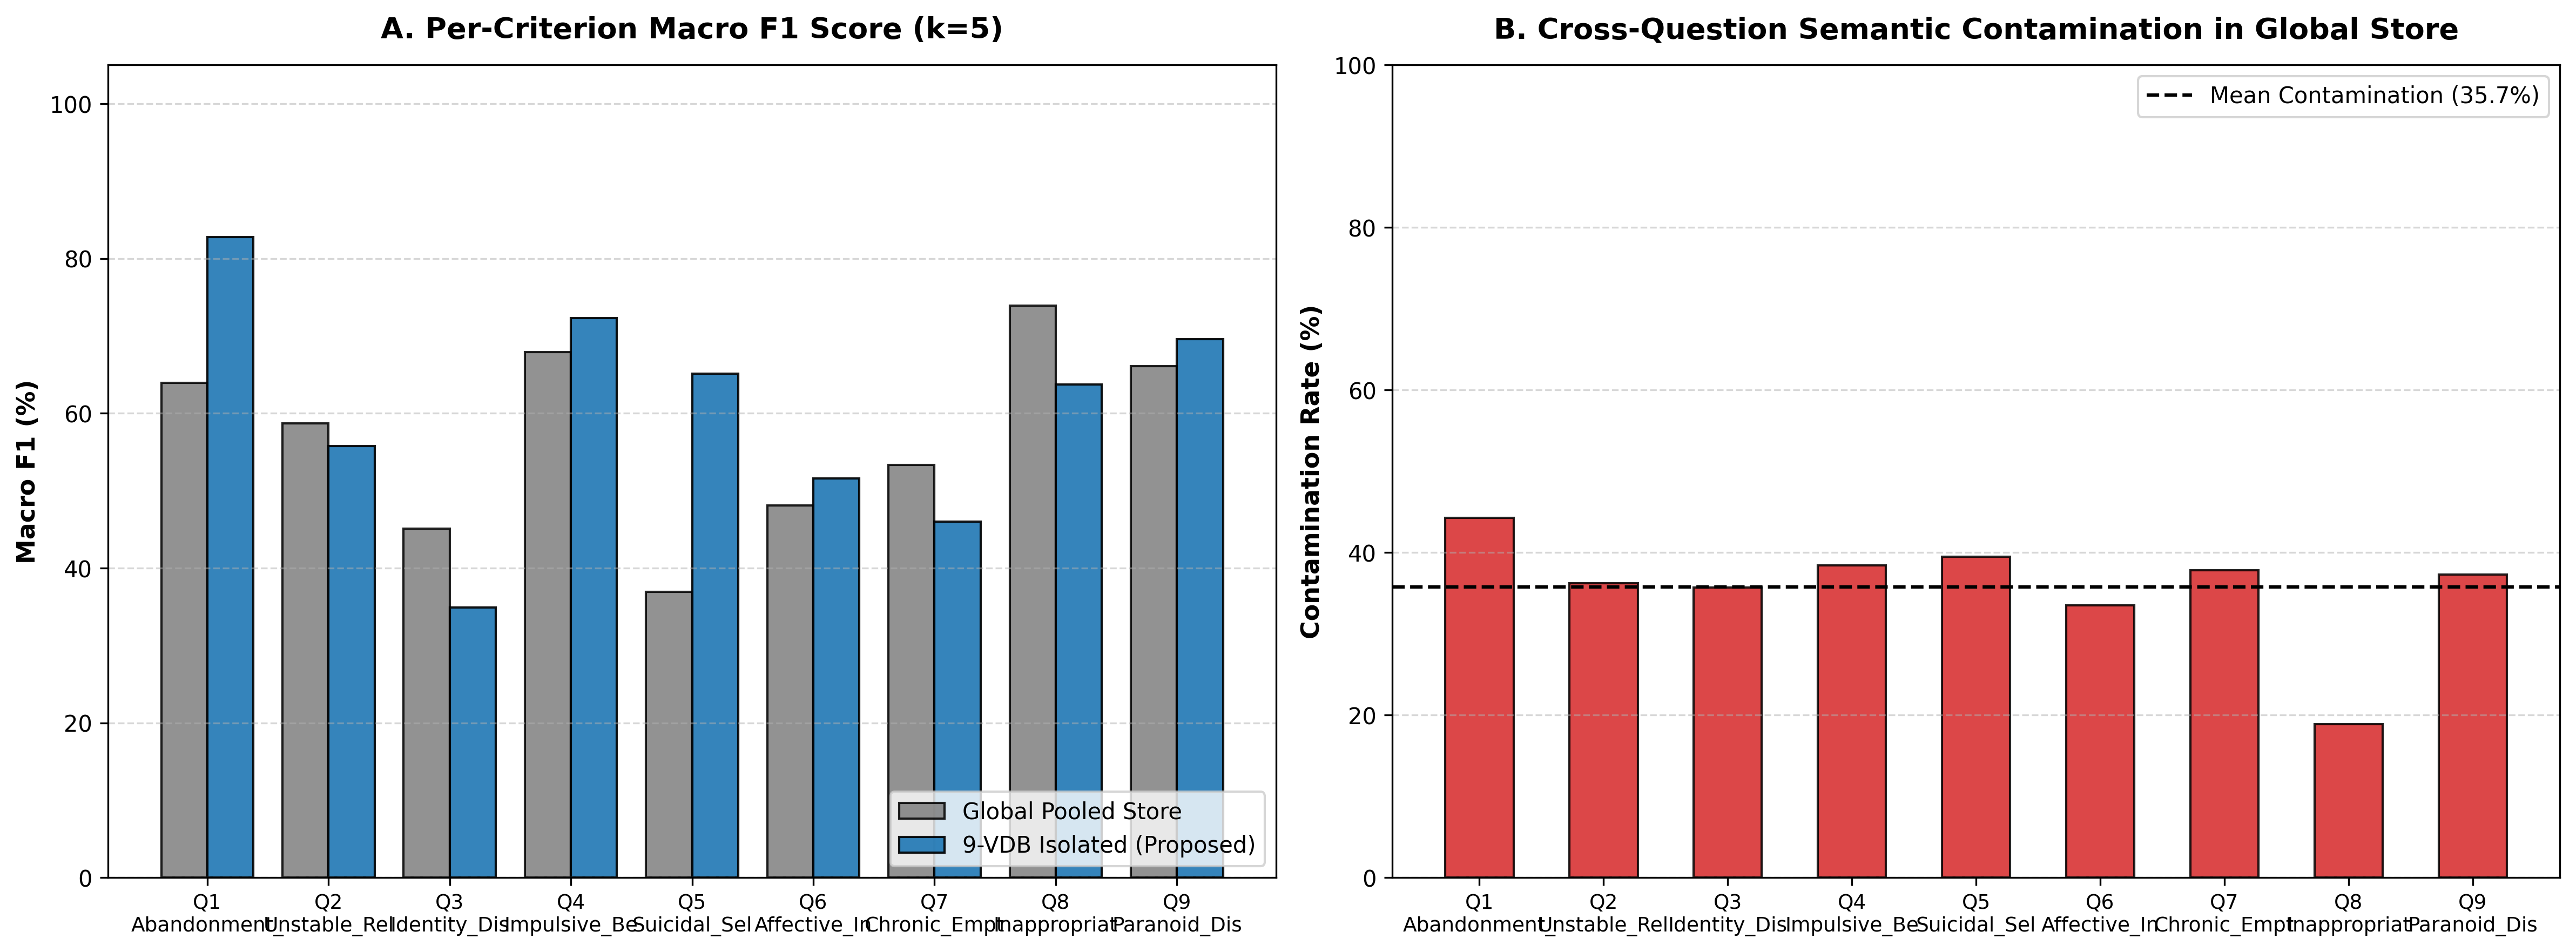
\includegraphics[width=\textwidth]{figures/vbri/imbalance_free_9_vdb_benchmark.png}
\caption{(a) Macro F1 per criterion for the pooled store and \vbri{} (9-VDB). (b) Share of
retrieved neighbours that come from the wrong criterion in the pooled store. For \vbri{} it is 0\%
by design.}
\label{fig:contam}
\end{figure}

\subsection{What makes semantic search work: a $2\times2$ ablation}

Table~\ref{tab:ablation} and Figure~\ref{fig:ablation} separate the two design decisions. First,
take the original training data, which is unbalanced inside each criterion. Isolating the criteria
barely helps here (65.47\% to 65.77\% accuracy). The vote inside each small database is dominated by
its majority class. Balancing the pooled store alone helps a little (67.87\%). Only the two
together give a large gain: 72.67\% accuracy and 85.07\% BPD sensitivity. The two decisions fix two
different problems. One is evidence from the wrong criterion. The other is an unfair class prior.
Each one is weak without the other. Compared with the balanced pooled store, the gain is
statistically significant (McNemar: 29 answers fixed and 13 broken, $\chi^2=5.36$, $p=0.021$;
exact $p=0.020$).

\begin{table}[H]
\centering
\caption{Ablation of \vbri{} design decisions (BGE-base, answer-only, $k=5$, $N=333$).
``Unbalanced'' uses the augmented training data with its natural per-criterion class mix
(4,279 vectors). ``Balanced'' uses 150 answers per class per criterion (4,050 vectors).}
\label{tab:ablation}
\small
\setlength{\tabcolsep}{5pt}
\resizebox{\textwidth}{!}{%
\begin{tabular}{@{}lccccc@{}}
\toprule
\textbf{Configuration} & \textbf{Isolation} & \textbf{Balance} & \textbf{Accuracy} & \textbf{Macro F1} & \textbf{BPD Sens.} \\
\midrule
Pooled store             & --          & --          & 65.47 & 57.07 & 67.16 \\
9 isolated stores        & \checkmark  & --          & 65.77 & 56.25 & --    \\
Pooled store             & --          & \checkmark  & 67.87 & 59.52 & 74.63 \\
\textbf{9 isolated stores (\vbri{} raw)} & \checkmark & \checkmark & \textbf{72.67} & \textbf{62.91} & \textbf{85.07} \\
\midrule
\quad + uncertainty margin ($\delta{=}0.05$, $\theta{=}0.45$) & \checkmark & \checkmark & 72.67 & 64.16 & 85.07 \\
\quad + C-SSRS safety rule (\vbri{} hybrid)                  & \checkmark & \checkmark & 72.97 & 64.48 & 86.57 \\
\bottomrule
\end{tabular}}
\end{table}

\begin{figure}[H]
\centering
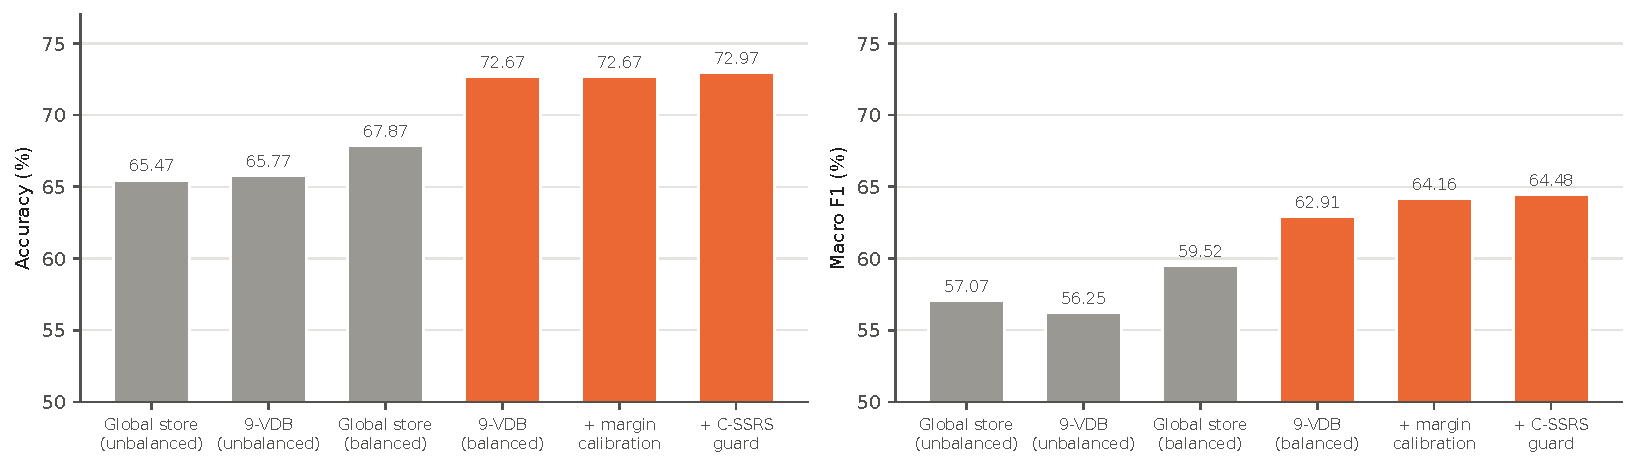
\includegraphics[width=\textwidth]{figures/generated/ablation_progression.pdf}
\caption{Accuracy and macro F1 as the \vbri{} design decisions are added. Grey bars miss at least
one of the two key decisions (isolation and balance). Orange bars have both.}
\label{fig:ablation}
\end{figure}

The two optional steps add little. The uncertainty margin changes six predictions. Three are fixed
and three are broken (exact McNemar $p=1.00$). It moves them into the Inconclusive class. This
raises Inconclusive recall from 39.0\% to 46.3\%, and macro F1 by 1.25 points. The C-SSRS rule fired
on exactly one test answer. It was a true suicide-attempt disclosure (``I did try to hang myself
from the ceiling fan'') that the vote had called Normal. It fired on no Normal or Inconclusive
answer. One correct override cannot prove that the rule works. But it shows why a safety check makes
sense for the most critical criterion.

Figure~\ref{fig:ksweep} shows that the choice of $k$ is not delicate. \vbri{} beats the pooled store
for every $k$ from 1 to 7. The best range is $k=3$ to 5. For larger $k$, the isolated databases
start to include less similar answers, and the advantage is lost.

\begin{figure}[H]
\centering
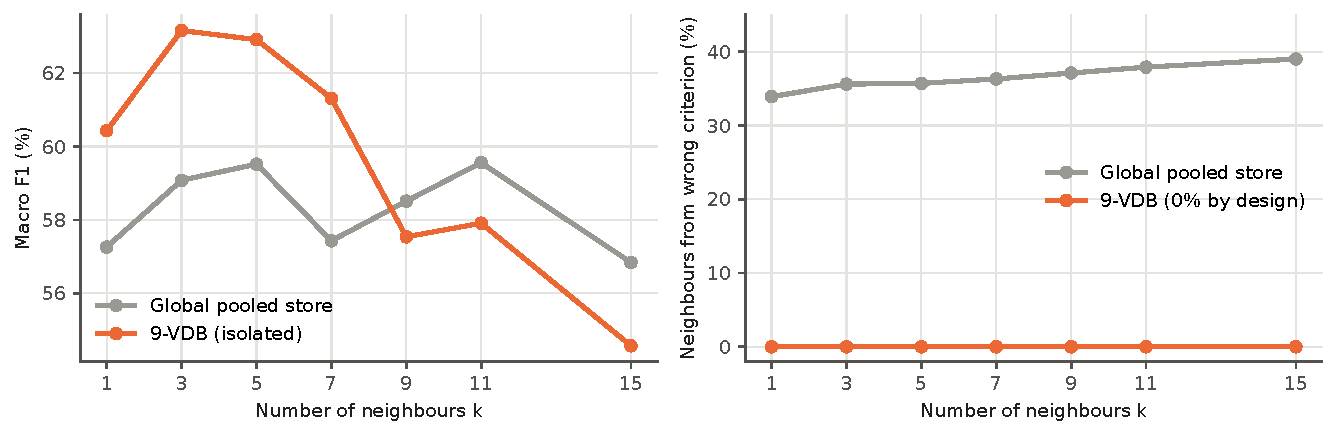
\includegraphics[width=0.85\textwidth]{figures/generated/k_sweep.pdf}
\caption{Sensitivity to the number of neighbours $k$. Left: macro F1. Right: share of
neighbours retrieved from the wrong criterion.}
\label{fig:ksweep}
\end{figure}

\subsection{Head-to-head: fine-tuning versus semantic search}

Table~\ref{tab:master} and Figure~\ref{fig:effect} place all configurations side by side.

\begin{table}[H]
\centering
\caption{All configurations on the same test set ($N=333$). ``Contam.'' is the share of retrieved
neighbours from the wrong criterion. It does not apply to fine-tuned models. Values in \%.}
\label{tab:master}
\scriptsize
\setlength{\tabcolsep}{3pt}
\renewcommand{\arraystretch}{1.2}
\resizebox{\textwidth}{!}{%
\begin{tabular}{@{}llcccccccc@{}}
\toprule
\textbf{Paradigm} & \textbf{Model} & \textbf{Params} & \makecell{\textbf{Trainable}\\\textbf{params}} &
\textbf{Contam.} & \textbf{Accuracy} & \textbf{Weighted F1} & \textbf{Macro F1} & \textbf{BPD Sens.} & \textbf{BPD F1} \\
\midrule
\multirow{6}{*}{\makecell[l]{Fine-tuned\\encoders}}
 & ModernBERT-base & 149M & 149M & N/A & \textbf{85.89} & \textbf{86.16} & \textbf{80.25} & \textbf{86.57} & \textbf{77.85} \\
 & ELECTRA-base    & 110M & 110M & N/A & 83.48 & 83.90 & 77.43 & \textbf{86.57} & 76.32 \\
 & RoBERTa-base    & 125M & 125M & N/A & 81.08 & 81.96 & 74.65 & 85.07 & 73.55 \\
 & BERT-base       & 110M & 110M & N/A & 79.58 & 80.28 & 74.80 & 80.60 & 69.23 \\
 & XLNet-base      & 117M & 117M & N/A & 77.48 & 78.32 & 71.01 & 85.07 & 65.90 \\
 & DistilBERT      & 66M  & 66M  & N/A & 74.77 & 76.14 & 69.67 & 83.58 & 65.88 \\
\midrule
\multirow{6}{*}{\makecell[l]{Pooled dense\\retrieval}}
 & BGE-base (Ans, balanced) & 109M & 0 & 35.7 & 67.87 & 69.82 & 59.52 & 74.63 & 56.50 \\
 & MPNet (Q+A)         & 109M & 0 & 36.2 & 67.57 & 68.71 & 57.28 & 68.66 & 50.89 \\
 & BGE-base (Ans)      & 109M & 0 & 35.5 & 65.47 & 67.52 & 57.07 & 67.16 & 55.43 \\
 & MPNet (Ans)         & 109M & 0 & 36.0 & 64.26 & 66.03 & 55.01 & 65.67 & 52.51 \\
 & PubMedBERT (Ans)    & 110M & 0 & 34.8 & 61.56 & 63.99 & 51.91 & 64.18 & 53.63 \\
 & MiniLM (Ans)        & 22M  & 0 & 35.1 & 60.66 & 62.84 & 52.51 & 58.21 & 42.39 \\
\midrule
\multirow{2}{*}{Lexical}
 & BM25 ($k{=}5$)   & 0 & 0 & 38.2 & 63.66 & 64.43 & 48.79 & 58.21 & 48.75 \\
 & TF-IDF ($k{=}5$) & 0 & 0 & 37.5 & 59.76 & 62.62 & 48.89 & 52.24 & 43.06 \\
\midrule
\multirow{3}{*}{\makecell[l]{\textbf{\vbri{}}\\\textbf{(ours)}}}
 & \textbf{9-VDB raw}   & 109M & \textbf{0} & \textbf{0.0} & 72.67 & 73.38 & 62.91 & 85.07 & 64.41 \\
 & 9-VDB calibrated     & 109M & \textbf{0} & \textbf{0.0} & 72.67 & 73.72 & 64.16 & 85.07 & 64.77 \\
 & 9-VDB hybrid         & 109M & \textbf{0} & \textbf{0.0} & 72.97 & 74.01 & 64.48 & \textbf{86.57} & 65.54 \\
\bottomrule
\end{tabular}}
\end{table}

\begin{figure}[H]
\centering
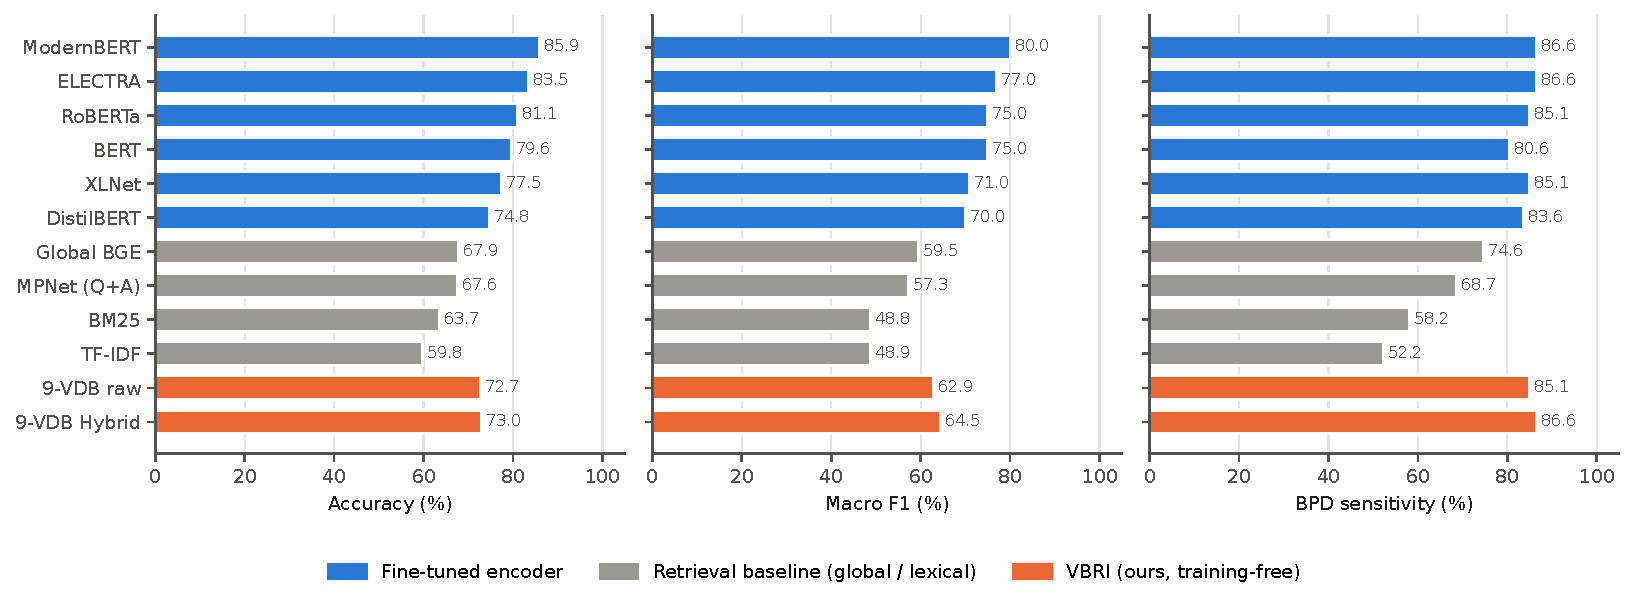
\includegraphics[width=\textwidth]{figures/generated/effectiveness_comparison.pdf}
\caption{Accuracy, macro F1 and BPD sensitivity of fine-tuned encoders (blue), pooled retrieval
baselines (grey) and \vbri{} (orange). On BPD sensitivity, training-free \vbri{} sits with the
best fine-tuned models. On accuracy and macro F1, it sits between them and the baselines.}
\label{fig:effect}
\end{figure}

Three findings stand out.

\textbf{(1) On BPD sensitivity, semantic search is close to fine-tuning (RQ1).} With no training,
\vbri{} finds 57 of the 67 BPD answers (85.07\%). ModernBERT and ELECTRA find 58. RoBERTa and XLNet
also find 57. With the C-SSRS rule, \vbri{} finds 58. It does better than BERT-base (80.60\%) and
DistilBERT (83.58\%) on this metric.

\textbf{(2) On overall accuracy, fine-tuning still wins by a clear margin.} ModernBERT is 13.2
points more accurate (85.89\% vs.\ 72.67\%). Its macro F1 is 17.3 points higher. The confusion
matrices in Figure~\ref{fig:h2h} show where the gap comes from. \vbri{} labels 41 Normal answers as
BPD (ModernBERT: 17). It also finds fewer Inconclusive answers (16 vs.\ 29). Semantic search is
good at finding answers that \emph{sound like} BPD answers. A trained decision boundary is better at
separating ordinary distress and vague answers from true pathology.

\textbf{(3) Structure matters more than the encoder.} Every pooled baseline stays below 68\%
accuracy and 75\% BPD sensitivity, whatever its encoder. The same BGE encoder gains about 5 points
of accuracy and 10 points of BPD sensitivity from isolation and balance alone.

\begin{figure}[H]
\centering
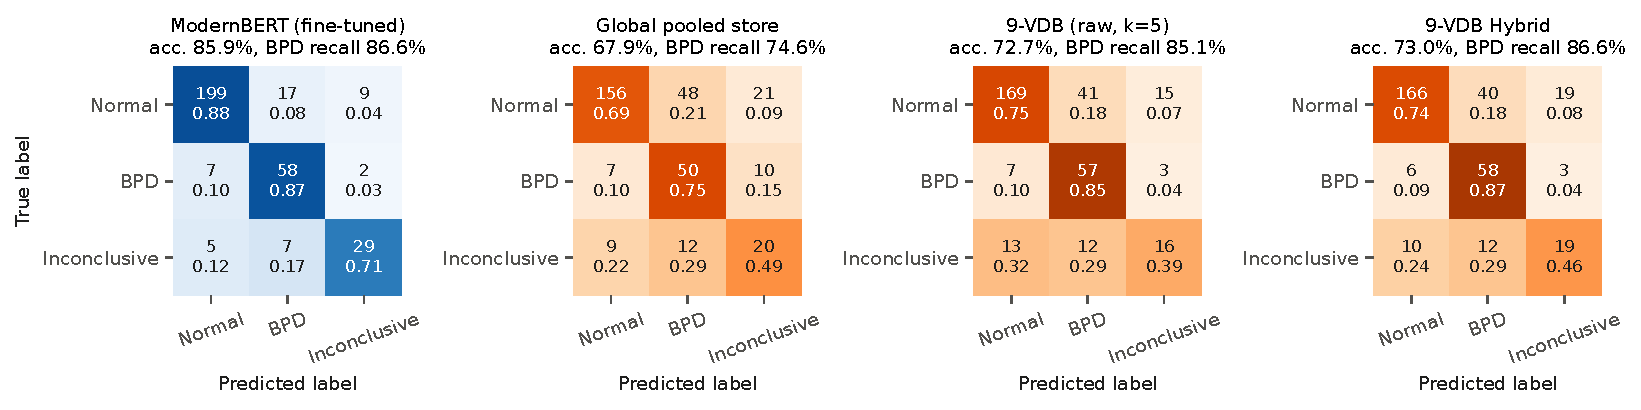
\includegraphics[width=\textwidth]{figures/generated/head_to_head_confusion.pdf}
\caption{Test confusion matrices of the best fine-tuned model (blue) and three semantic search
configurations (orange). Moving from the pooled store to \vbri{} mainly recovers BPD answers.
ModernBERT is still better at keeping Normal and Inconclusive answers apart from BPD.}
\label{fig:h2h}
\end{figure}

\subsection{What fine-tuning costs and what semantic search saves}

Table~\ref{tab:cost} and Figure~\ref{fig:cost} answer RQ2.

\begin{table}[H]
\centering
\caption{Computational cost of building and running each classifier. Inference time is per answer
with batched inputs on a Tesla T4. Storage is what must be kept for this task only (fp32 weights,
or the vector index). The frozen \vbri{} encoder (109M parameters) is shared across tasks, so it is
not counted.}
\label{tab:cost}
\small
\setlength{\tabcolsep}{5pt}
\resizebox{\textwidth}{!}{%
\begin{tabular}{@{}lccccc@{}}
\toprule
\textbf{Model} & \makecell{\textbf{Gradient}\\\textbf{updates}} & \makecell{\textbf{Training /}\\\textbf{index build}} &
\makecell{\textbf{Inference}\\\textbf{per answer}} & \makecell{\textbf{Task-specific}\\\textbf{storage}} & \textbf{BPD Sens.} \\
\midrule
ModernBERT-base & Yes & 179\,s   & 4.10\,ms  & 596\,MB & 86.57 \\
ELECTRA-base    & Yes & 1,062\,s & 9.46\,ms  & 440\,MB & 86.57 \\
RoBERTa-base    & Yes & 668\,s   & 8.62\,ms  & 500\,MB & 85.07 \\
BERT-base       & Yes & 1,066\,s & 8.96\,ms  & 440\,MB & 80.60 \\
XLNet-base      & Yes & 666\,s   & 12.55\,ms & 468\,MB & 85.07 \\
DistilBERT      & Yes & 475\,s   & 4.54\,ms  & 264\,MB & 83.58 \\
\midrule
\textbf{\vbri{} (9-VDB raw)} & \textbf{No} & \textbf{12\,s} & \textbf{2.39\,ms} & \textbf{12.4\,MB} & 85.07 \\
\quad of which: query encoding / search & & & 2.31 / 0.08\,ms & & \\
\bottomrule
\end{tabular}}
\end{table}

\begin{figure}[H]
\centering
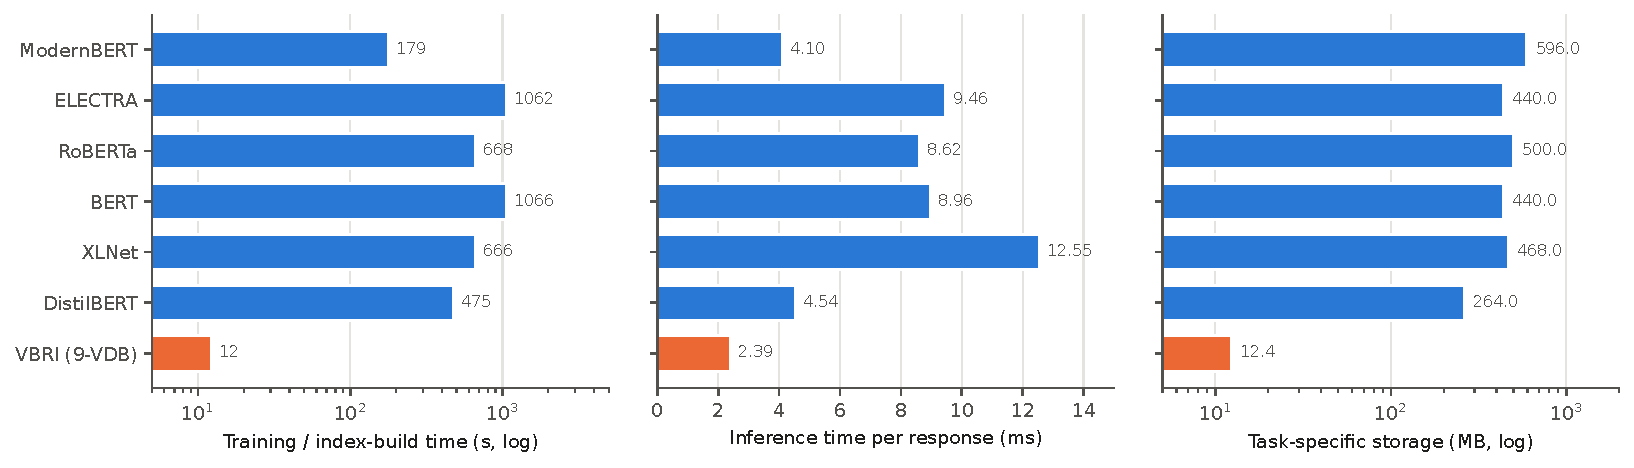
\includegraphics[width=\textwidth]{figures/generated/cost_comparison.pdf}
\caption{Cost of each classifier: time to train (fine-tuning) or to build the index (\vbri{}),
inference time per answer, and task-specific storage. The first and third panels use
logarithmic scales.}
\label{fig:cost}
\end{figure}

The biggest saving is in \emph{building} the classifier. Fine-tuning took 3 to 18 minutes per model
on a GPU. Finding a good setup needed many such runs. We tried three learning rates and three ways
of handling class imbalance. We also repeated runs for unstable models such as DeBERTa. \vbri{}
needs one pass of the frozen encoder over 4,050 answers. This took 12.25\,s. There are no gradient
updates, and no search over learning rate or number of epochs. That is about 15 times faster than
the quickest fine-tuning run. It is about 87 times faster than BERT or ELECTRA.

The task-specific \emph{storage} is 48 times smaller than a ModernBERT checkpoint (12.4\,MB vs.\
596\,MB). The encoder is shared and frozen. So a second screening task needs a second small index,
not a second copy of a large model. When clinicians label new answers, we insert rows. We do not
retrain.

At \emph{inference}, \vbri{} needs 2.39\,ms per answer. Only 0.08\,ms of that is the search itself.
It is 1.7 times faster than ModernBERT, and about 4 times faster than ELECTRA or BERT. The search
is so cheap that the cost of \vbri{} is mostly the cost of running one embedding model once per
answer. It would stay cheap even with many more stored answers.

\subsection{Per-criterion behaviour}

Table~\ref{tab:per_criterion} and Figure~\ref{fig:vdb_cm} break the \vbri{} result down by question.
The biggest gains over the pooled store are for abandonment (Q1: +13.5 points accuracy, +20.2 points
BPD F1) and suicidal and self-harm behaviour (Q5: +13.5 points accuracy). These two criteria
suffered most from contamination. Identity disturbance (Q3) stays the hardest. Normal questioning of
one's goals and pathological identity disturbance use very similar words. Ten of the 29 Normal
answers to Q3 were labelled BPD.

\begin{table}[H]
\centering
\caption{Per-criterion comparison of the pooled store and \vbri{} (9-VDB raw), $N=37$ per
criterion. Values in \%.}
\label{tab:per_criterion}
\scriptsize
\setlength{\tabcolsep}{3pt}
\renewcommand{\arraystretch}{1.1}
\resizebox{\textwidth}{!}{%
\begin{tabular}{@{}clccccccc@{}}
\toprule
\textbf{Q\#} & \textbf{DSM-5 criterion} & \textbf{Contam.} &
\textbf{Pooled acc.} & \textbf{9-VDB acc.} & \textbf{$\Delta$ acc.} &
\textbf{Pooled BPD F1} & \textbf{9-VDB BPD F1} & \textbf{$\Delta$ BPD F1} \\
\midrule
Q1 & Abandonment avoidance  & 44.3 & 67.6 & \textbf{81.1} & \textbf{+13.5} & 58.3 & \textbf{78.6} & \textbf{+20.2} \\
Q2 & Unstable relationships & 36.2 & 67.6 & 64.9 & $-$2.7 & 50.0 & 55.6 & +5.6  \\
Q3 & Identity disturbance   & 35.7 & 59.5 & 59.5 & 0.0    & 31.6 & 28.6 & $-$3.0 \\
Q4 & Impulsive behaviours   & 38.4 & 81.1 & \textbf{83.8} & +2.7 & 54.5 & 54.5 & 0.0 \\
Q5 & Suicidal / self-harm   & 39.5 & 75.7 & \textbf{89.2} & \textbf{+13.5} & 22.2 & \textbf{33.3} & \textbf{+11.1} \\
Q6 & Affective instability  & 33.5 & 51.4 & \textbf{59.5} & +8.1 & 69.2 & \textbf{75.0} & +5.8 \\
Q7 & Chronic emptiness      & 37.8 & 56.8 & \textbf{62.2} & +5.4 & 53.8 & \textbf{66.7} & \textbf{+12.8} \\
Q8 & Inappropriate anger    & 18.9 & 78.4 & 75.7 & $-$2.7 & 69.2 & \textbf{76.9} & +7.7 \\
Q9 & Paranoia / dissociation& 37.3 & 73.0 & \textbf{78.4} & +5.4 & 70.0 & \textbf{73.7} & +3.7 \\
\midrule
\multicolumn{2}{l}{\textbf{Overall}} & \textbf{35.7} & \textbf{67.9} & \textbf{72.7} & \textbf{+4.8} &
\textbf{56.5} & \textbf{64.4} & \textbf{+7.9} \\
\bottomrule
\end{tabular}}
\end{table}

\begin{figure}[H]
\centering
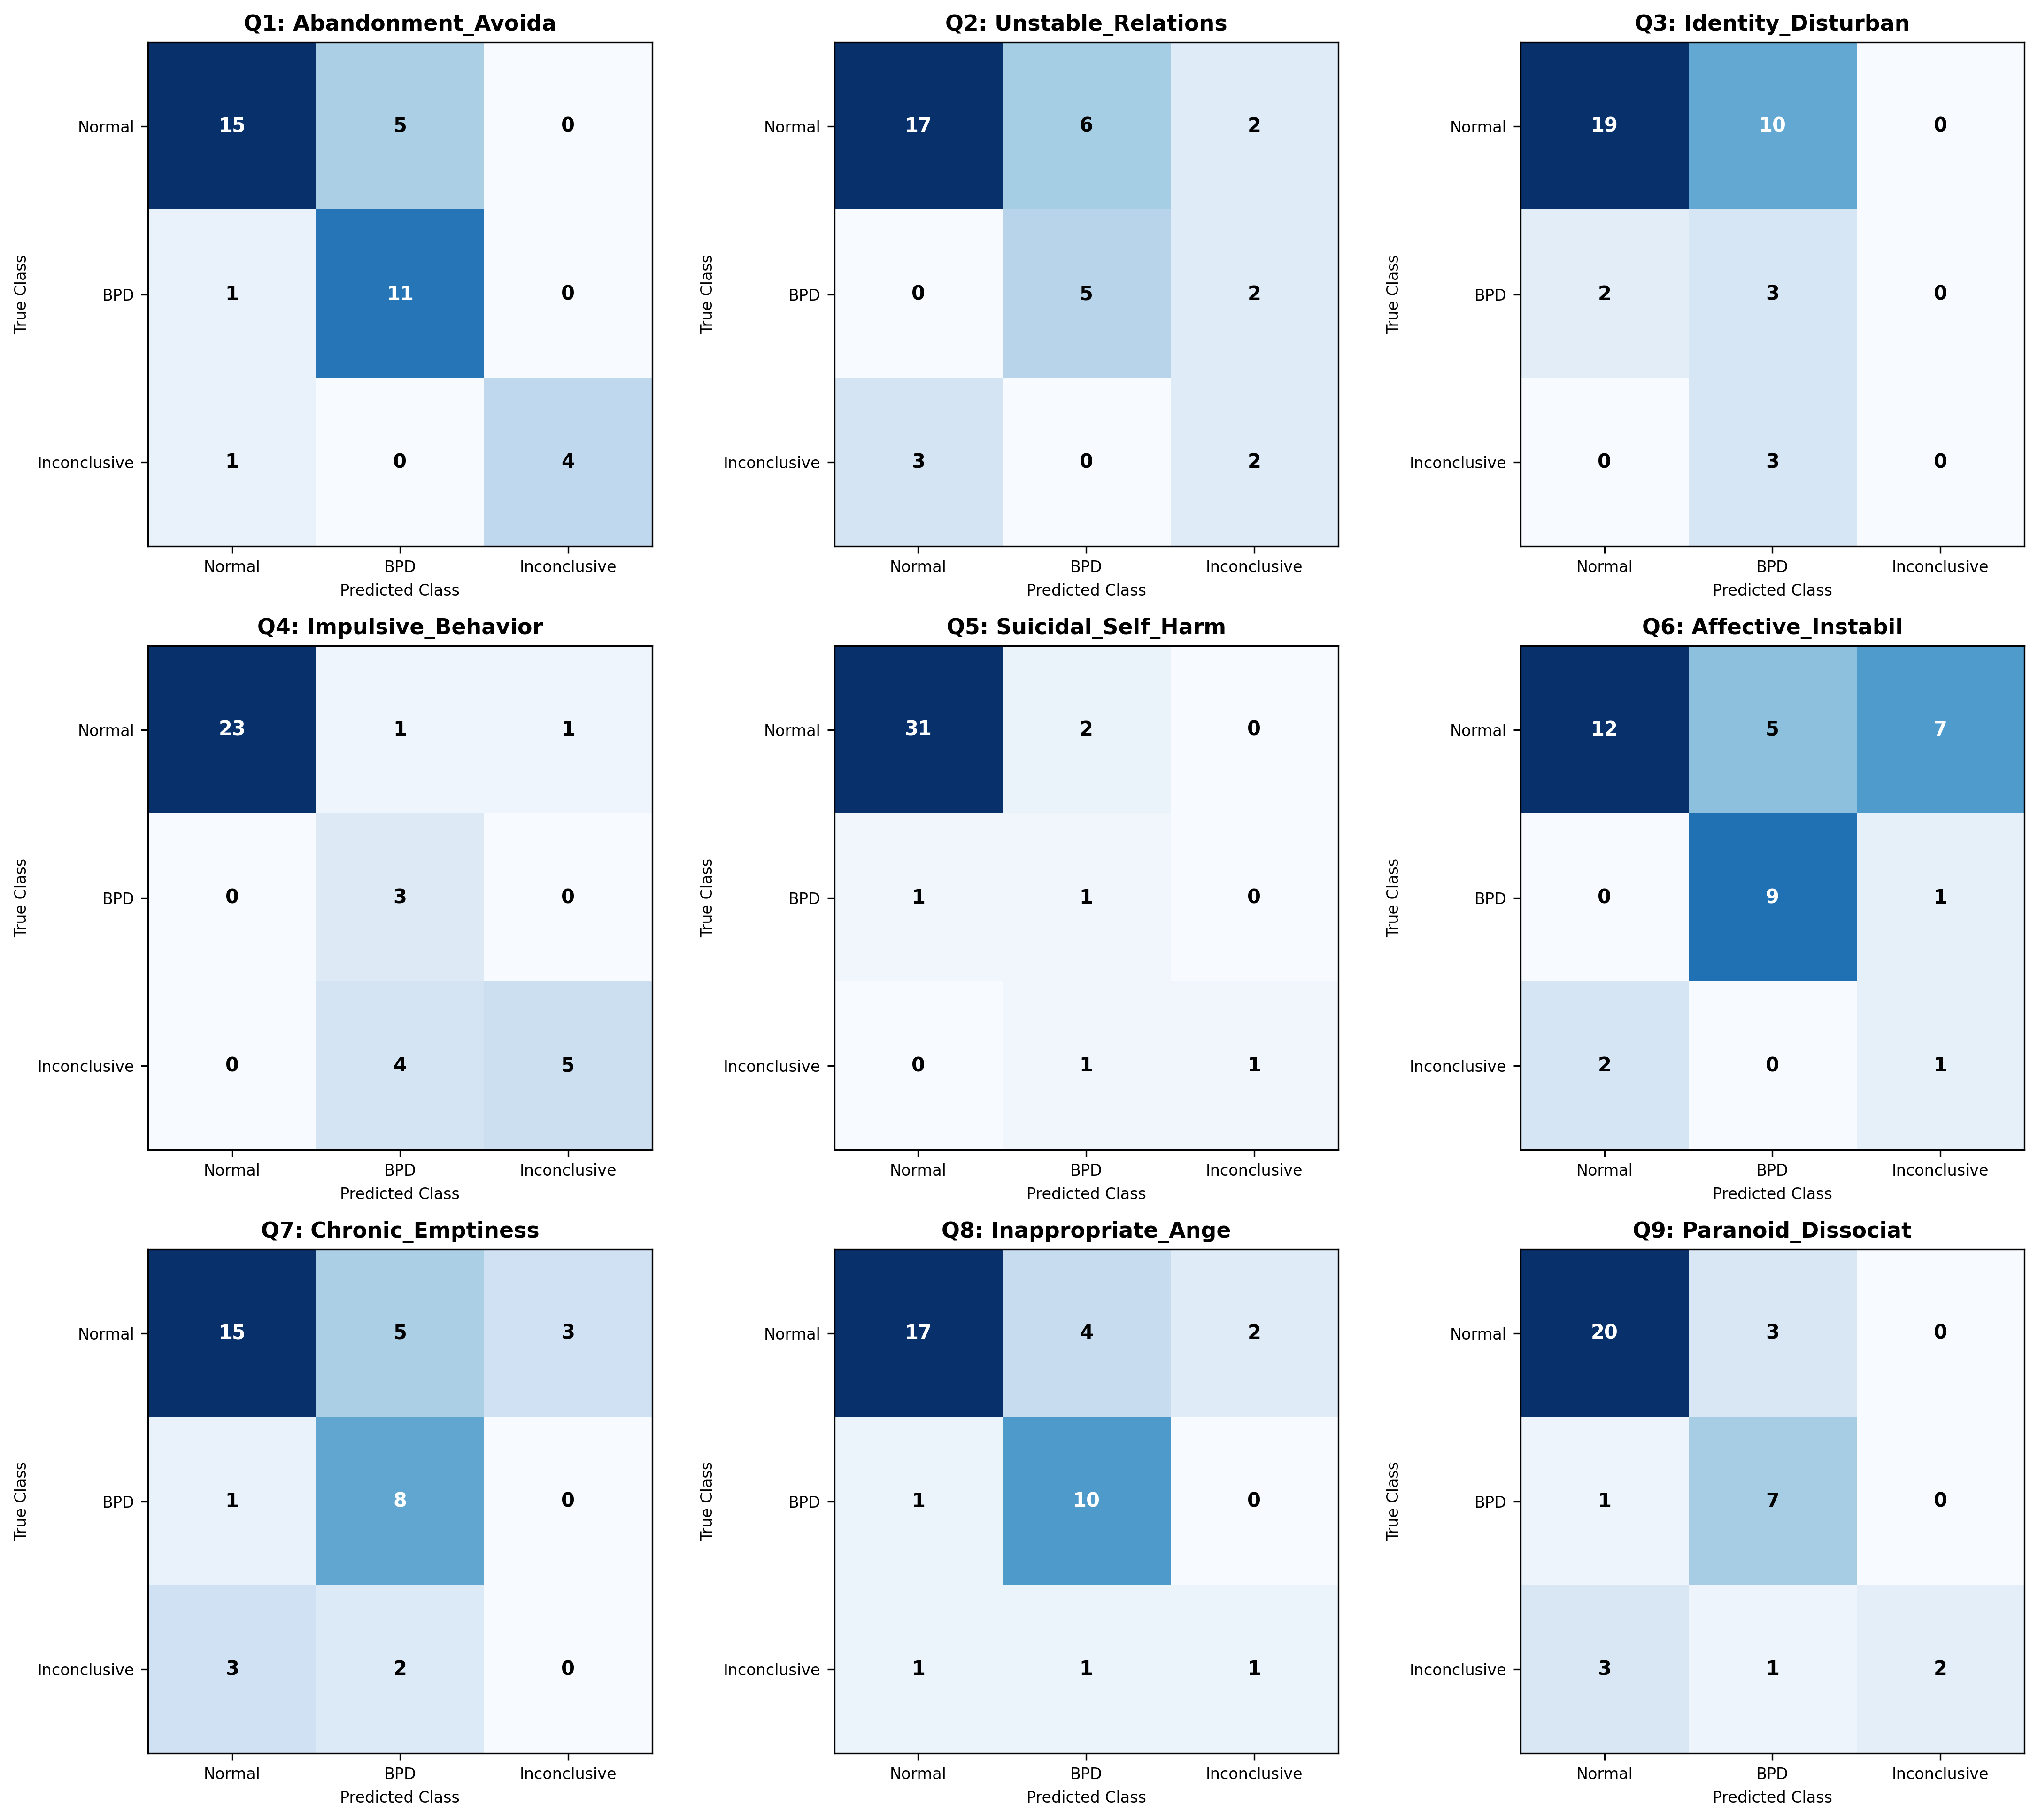
\includegraphics[width=0.9\textwidth]{figures/vbri/confusion_matrices_9_vdb.png}
\caption{\vbri{} confusion matrices for each of the nine \dsmv{} criteria (test set, 37 answers
each).}
\label{fig:vdb_cm}
\end{figure}

Across the nine criteria, the mean accuracy gain of \vbri{} over the pooled store is +4.8 points
(paired test over criteria, $p=0.047$). Figure~\ref{fig:calib} shows the effect of the uncertainty
margin on the confusion matrix.

\begin{figure}[H]
\centering
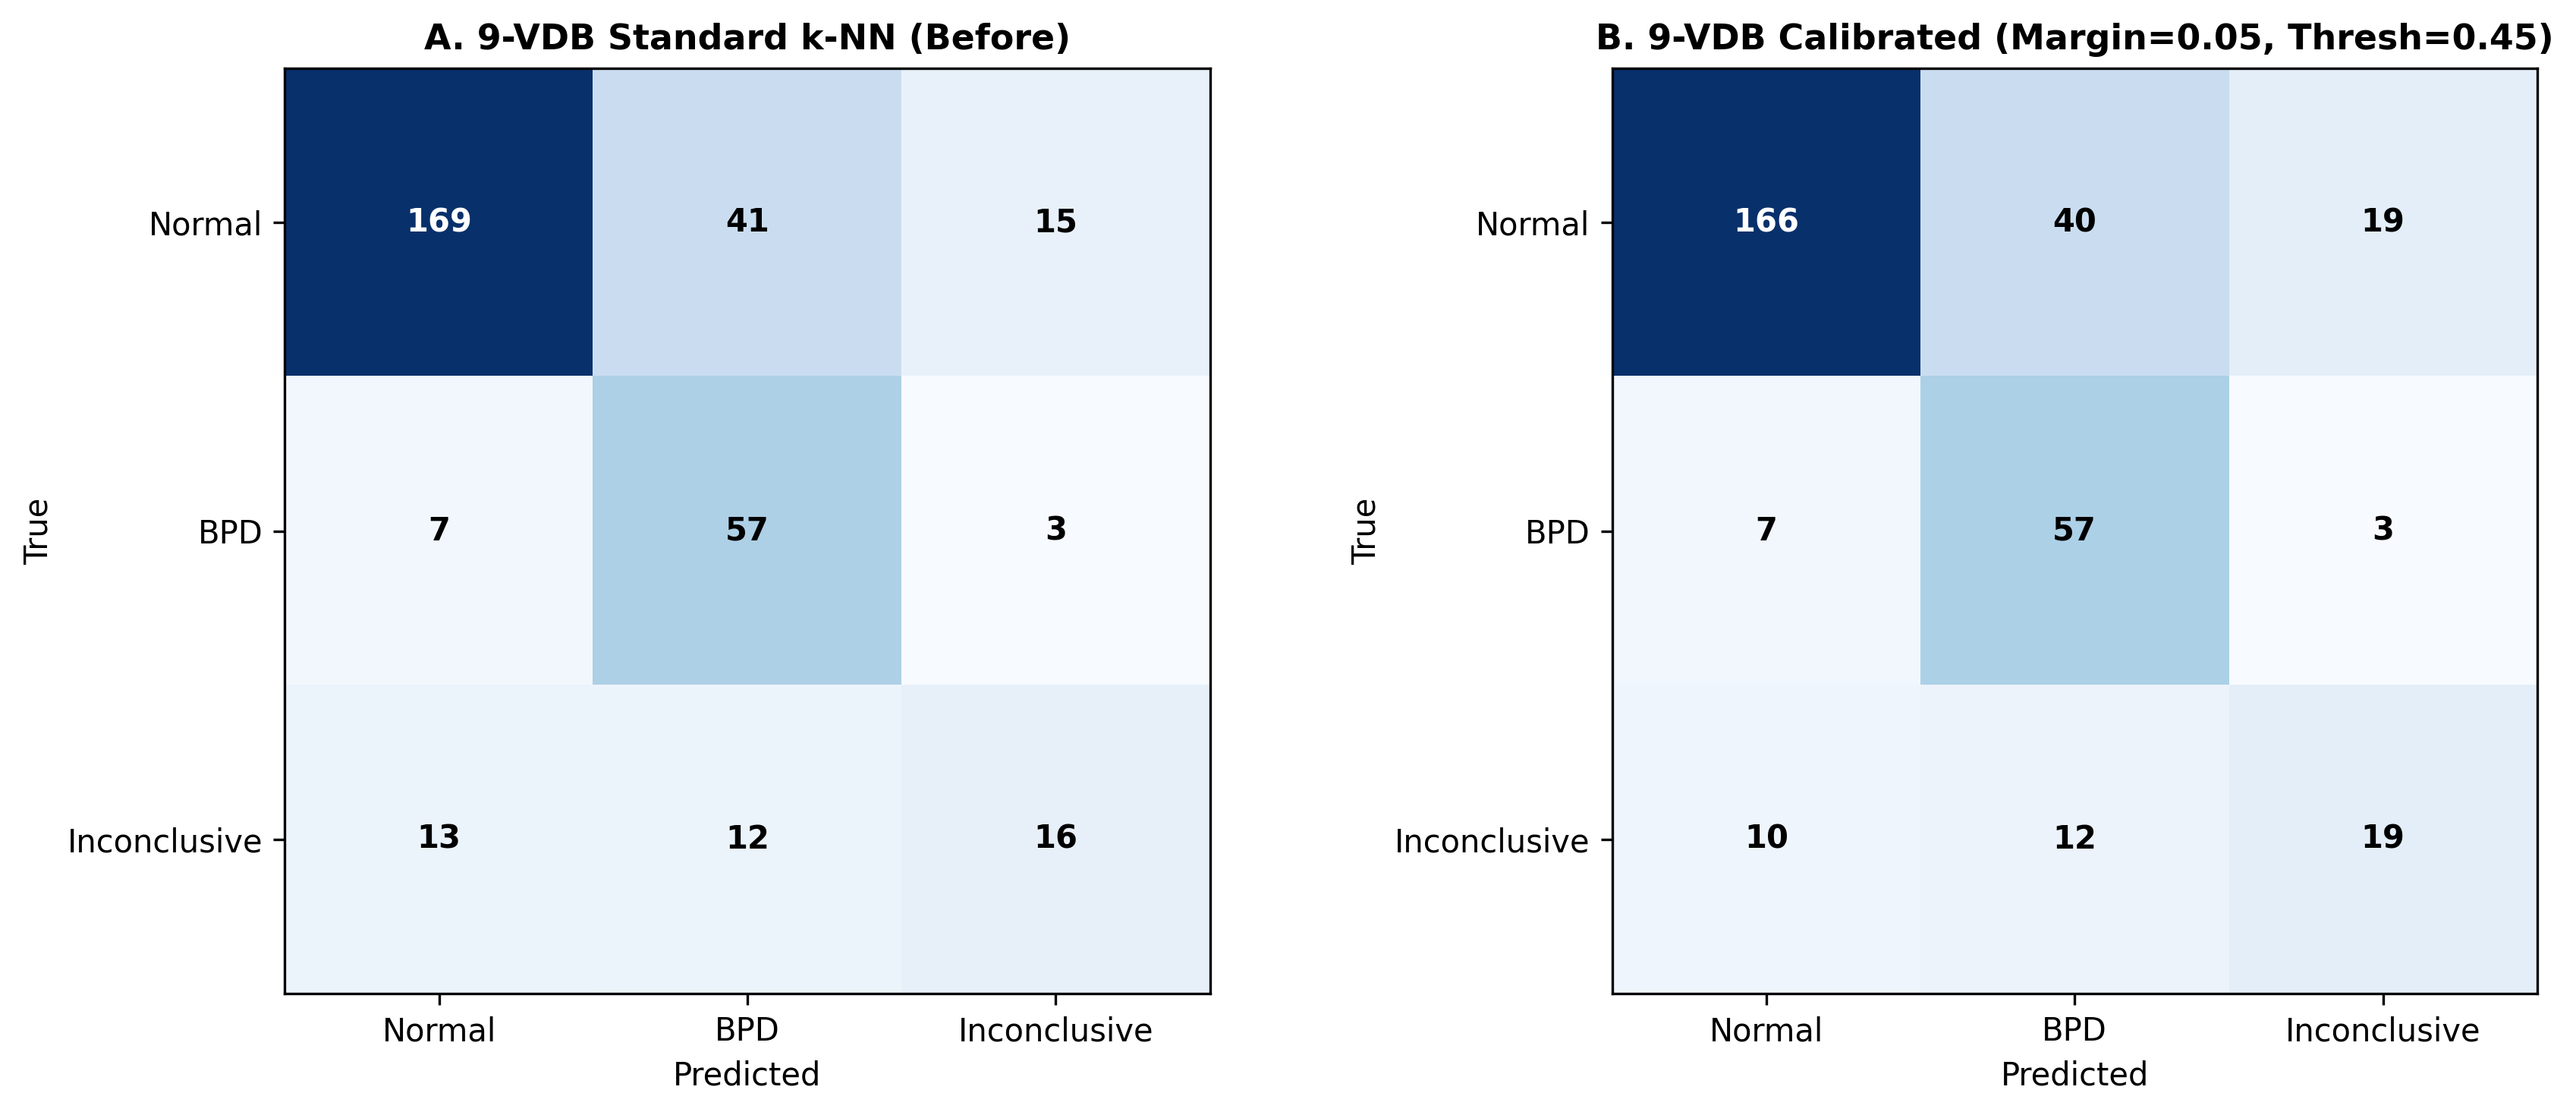
\includegraphics[width=0.8\textwidth]{figures/vbri/calibration_before_after_confusion.png}
\caption{\vbri{} confusion matrix before (left) and after (right) the uncertainty margin. The
margin moves a few uncertain answers into the Inconclusive class.}
\label{fig:calib}
\end{figure}

\subsection{Explainability: every decision comes with its evidence}

\vbri{} classifies by retrieval. So each prediction can be shown with the stored answers that
produced it. Table~\ref{tab:vignettes} gives three test cases. In the first, the pooled store called
a healthy answer BPD. Three of its five neighbours came from other questions. \vbri{} retrieved
only paranoia and dissociation answers, and got it right. In the second, an evasive answer gave
nearly equal class scores. It was flagged as Inconclusive. A fine-tuned model can only give
explanations after the fact. For \vbri{}, the explanation is the evidence that was actually used.

\begin{table}[H]
\centering
\caption{Clinical vignettes from the test set. They show how retrieval exposes its reasoning.}
\label{tab:vignettes}
\small
\setlength{\tabcolsep}{4pt}
\resizebox{\textwidth}{!}{%
\begin{tabular}{@{}p{1.1cm}p{5.6cm}p{1.7cm}p{1.8cm}p{4.2cm}@{}}
\toprule
\textbf{Q} & \textbf{Answer (excerpt)} & \textbf{True label} & \textbf{Prediction} & \textbf{What the retrieval shows} \\
\midrule
Q9 & ``I feel overly attached to my reality. I know the things I must do\ldots'' & Normal &
  Pooled: BPD\newline \vbri{}: Normal & Pooled store: 60\% of neighbours from other criteria.
  \vbri{}: neighbours only from Q9. \\
Q7 & ``I do not feel like talking about this\ldots'' & Inconclusive & \vbri{}: Inconclusive &
  Top two class scores within the margin $\delta=0.05$. Flagged as ambiguous. \\
Q1 & ``Sometimes it's important to prevent the close one from leaving us\ldots'' & BPD &
  \vbri{}: BPD & Neighbours agree with labelled abandonment-avoidance answers. \\
\bottomrule
\end{tabular}}
\end{table}

\subsection{Binary screening and participant-level agreement}

In practice, a screening tool often answers one question: should this person be referred? To test
this, we treat BPD as positive and the other two labels as negative (Table~\ref{tab:screening}).

\begin{table}[H]
\centering
\caption{Binary screening view (BPD vs.\ not BPD) on the test set ($N=333$, 67 positive). Values in \%.}
\label{tab:screening}
\small
\begin{tabular}{@{}lcccccc@{}}
\toprule
\textbf{Model} & \textbf{Accuracy} & \textbf{Sensitivity} & \textbf{Specificity} & \textbf{PPV} & \textbf{NPV} & \textbf{DOR} \\
\midrule
ModernBERT (fine-tuned) & \textbf{90.09} & \textbf{86.57} & \textbf{90.98} & \textbf{70.73} & \textbf{96.41} & \textbf{65.0} \\
\vbri{} raw             & 81.08 & 85.07 & 80.08 & 51.82 & 95.52 & 22.9 \\
\vbri{} hybrid          & 81.68 & \textbf{86.57} & 80.45 & 52.73 & 95.96 & 26.5 \\
Pooled BGE store        & 76.88 & 74.63 & 77.44 & 45.45 & 92.38 & 10.1 \\
\bottomrule
\end{tabular}
\end{table}

Both \vbri{} and ModernBERT have a negative predictive value above 95\%. When either one clears an
answer, it is almost always right. The difference is in specificity. ModernBERT raises fewer false
alarms (PPV 70.7\% vs.\ 52.7\%). With \vbri{}, about one in two positive flags is a true BPD answer.
For a first-line screen where a clinician reviews every positive, this is acceptable. For a
stand-alone decision, it is not.

We also checked participant-level agreement. There are 221 test participants, and each gave one to
five test answers. The number of criteria that \vbri{} marks as BPD agrees better with the expert
count than the pooled store does. The mean absolute error is 0.276 vs.\ 0.321. The Pearson
correlation is $r=0.60$ vs.\ $0.52$ (Figure~\ref{fig:patient_level}). No participant has more than
two BPD-labelled answers in the test split. So the \dsmv{} rule of five or more criteria cannot be
tested here.

\begin{figure}[H]
\centering
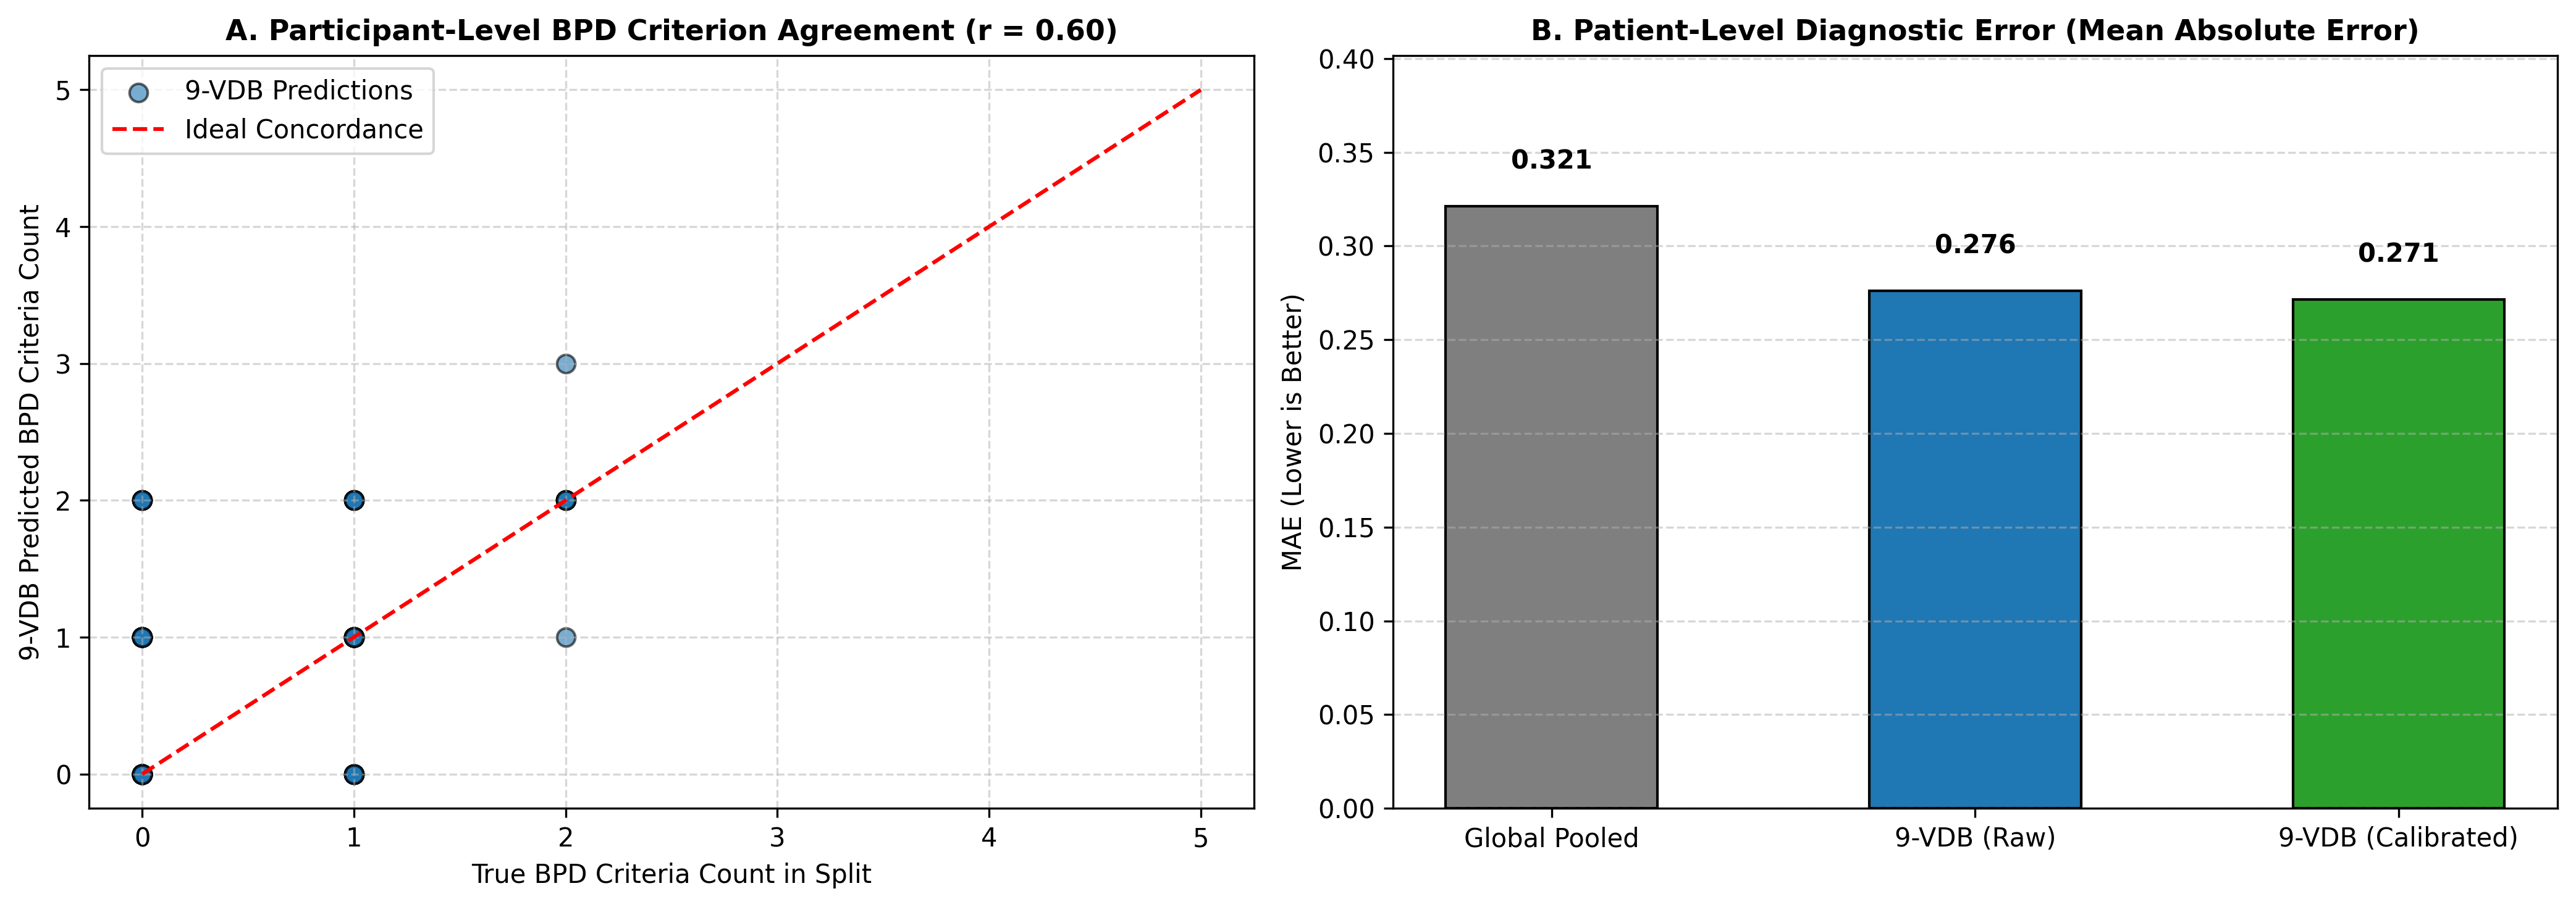
\includegraphics[width=0.85\textwidth]{figures/vbri/patient_level_diagnostic_agreement.png}
\caption{Participant-level agreement between predicted and expert-labelled BPD criterion counts
(221 test participants).}
\label{fig:patient_level}
\end{figure}

% =============================================================================
% 6. DISCUSSION
% =============================================================================
\section{Discussion}\label{sec:discussion}

\paragraph{So, do we need to fine-tune?}
It depends on what the classifier is for. Say the goal is the highest overall accuracy on all three
classes. Then yes. In our tests, a fine-tuned encoder is 13 points more accurate than semantic
search. It also separates Inconclusive answers much better. Now say the goal is a first-line screen
that rarely misses a BPD answer. It should be built in seconds. It should run on modest hardware and
update without retraining. A clinician should be able to see why it decided what it did. Then no. A
frozen embedding model with a well-built vector database reaches the same range of sensitivity as
the fine-tuned models (85.07\% vs.\ 86.57\%). It costs a small part of the price. So we do not
claim that semantic search replaces fine-tuning everywhere. We see it as a strong, practical default
for sensitivity-driven screening. Fine-tuning fits cases where its extra accuracy is worth the cost.

\paragraph{The index structure is the model.}
The most useful lesson is about \emph{how} to use semantic search for classification. A single
pooled index treated the nine criteria as one problem. Over a third of its evidence came from the
wrong question. Isolating each criterion and balancing each database did more than any change of
encoder. In a fine-tuned model, such issues are absorbed into the learned weights. In a retrieval
classifier, they must be handled by design. Any structured instrument with known item boundaries
can use the same recipe. Examples are psychiatric questionnaires, triage forms and symptom
checklists.

\paragraph{Relation to LLMs.}
We did not run generative LLMs. So our results do not measure them directly. The literature,
though, shows that prompted LLMs usually do not beat fine-tuned encoders on
classification~\cite{bucher2024finetuned,edwards2024icl,lho2025jama}. They also cost more to run, and
they raise privacy concerns for clinical text~\cite{guo2024llmreview}. \vbri{} reaches the
sensitivity range of the fine-tuned encoders. So it is reasonable to expect it to compete with
LLM-based screening on this kind of task, at a much lower cost. Testing this directly is an
important next step.

\paragraph{Limitations.}
This study has several limits. They should be addressed before any clinical use.
\begin{itemize}[leftmargin=*,itemsep=2pt]
  \item \emph{Selection on the held-out split.} We chose $k$, the margin, the threshold and the
        C-SSRS rule while looking at the held-out results. We reduced the effect in two ways. The raw
        configuration is the main result. And $k=3$ to 7 gives similar results. Still, all \vbri{}
        numbers should be confirmed with settings fixed on the validation set, and with a fresh
        test set.
  \item \emph{Negation and short disclosures.} \vbri{} raw made 91 errors. Of these, 41 were Normal
        answers labelled BPD. Of those 41, 23 contain an explicit negation (``never'', ``not'',
        ``nothing''). Their embeddings sit close to the affirmative versions. This is a known
        weakness of sentence encoders~\cite{chiang2023heros,cao2025negation}. Most of the others
        describe ordinary distress, for example anger at a real harassment incident, in the same
        words that pathological answers use. Negation-aware encoders or a light negation filter are
        natural fixes.
  \item \emph{One dataset, one language, one domain.} \bpdqac{} is a single English dataset with 362
        mostly student participants. The test set has 333 answers. With 67 BPD test answers, a
        one-answer difference in sensitivity is 1.5 points. Splits are at answer level. So one
        participant can have answers in both the training and test sets, for different questions.
  \item \emph{Augmented examples in the store.} Of the 4,050 stored answers, 1,800 are augmented
        texts. For rare classes, such as BPD answers to Q5, most stored examples are augmented. Their
        quality directly affects retrieval.
  \item \emph{Hardware.} All timings come from a Tesla T4 GPU. We did not measure CPU or mobile
        hardware. We expect the advantage of avoiding training to grow there, but this must still
        be shown.
\end{itemize}

% =============================================================================
% 7. CONCLUSION
% =============================================================================
\section{Conclusion}\label{sec:conclusion}

This paper asked a simple question. Must a clinical text classifier be fine-tuned, or can semantic
search over a frozen embedding model do the job? We tested this on structured BPD interview answers.
Our training-free classifier, \vbri{}, stores expert-labelled answers in nine criterion-isolated,
class-balanced vector databases. It labels new answers by similarity-weighted voting. With no
training at all, it finds 85.07\% of BPD answers. That is within one answer of the best fine-tuned
transformer. It replaces minutes of GPU fine-tuning with a 12-second indexing step. It needs a 12.4\,MB
index instead of a model of several hundred megabytes. It runs in 2.4\,ms per answer. And it shows
the evidence behind every decision. Fine-tuned models are still clearly better on overall accuracy
and on ambiguous answers. The practical message is clear. Fine-tuning should not be the automatic
first step. For sensitivity-focused screening in resource-constrained settings, a well-designed
semantic search index is a credible, cheaper and more transparent option. The design of that index
matters as much as the choice of embedding model.

\section*{Data Availability}

The \bpdqac{} dataset is available at \textless{}repository link\textgreater{} as a CSV file. It
contains unique identifiers, question texts, participant responses, expert-annotated labels and
binary indicators for Criteria B through F. The \vbri{} package is provided as supplementary
material. It includes model artefacts, per-criterion audit files, test predictions and the scripts
used to make the figures in this paper.

\printbibliography

\end{document}
